\chapter{Metric Spaces}

\section{Basic Definitions and Examples}
    \begin{definition}
        A \textit{metric} on a nonempty set $X$ is a map
            \begin{equation*}
            \begin{split}
                d: X \times X \rightarrow [0,\infty)
            \end{split}
            \end{equation*}
        satisfying for all $x,y,z \in X$:
            \begin{enumerate}[label = (\arabic*),itemsep=1pt,topsep=3pt]
                \item $d(x,y) = d(y,x)$ (symmetry);
                \item $d(x,z) \leq d(x,y) + d(y,z)$ (triangle inequality);
                \item $d(x,x) = 0$;
                \item if $d(x,y) = 0$ then $x=y$ (positivity).
            \end{enumerate}
        If $d$ satisfies all but (iv), then $d$ is called a \textit{semi-metric}. The pair $(X,d)$ is called a \textit{metric space}.
    \end{definition}

    \begin{definition}
        \phantom{a}
        \begin{enumerate}[label = (\arabic*),itemsep=1pt,topsep=3pt]
            \item Two metrics $d,\rho$ on $X$ are called \textit{equivalent} if there exists constants $c,c'$ with $d(x,y) \leq c \rho(x,y)$ and $\rho(x,y) \leq c'd(x,y)$.
            \item Let $\{d_k\}_{k=1}^\infty$ be a family of metrics on $X$. If for all $x,y \in X$ and $k \in \bfN$ we have $d_k(x,y) \leq C$, then we say the family of metrics is \textit{uniformly bounded}.
        \end{enumerate}
    \end{definition}

    \begin{example}
        \phantom{a}
        \begin{enumerate}[label = (\arabic*),itemsep=1pt,topsep=3pt]
            \item The \textit{discrete metric} on $X \neq \emptyset$ is:
                \begin{equation*}
                \begin{split}
                    d(x,y) = \begin{cases}1, & x \neq y \\ 0, & x =y  .\end{cases}
                \end{split}
                \end{equation*}

            \item The \textit{hamming distance} between two bit strings of equal length: given $X = \{0,1\}^n$, then $d_H:X \times X \rightarrow [0,\infty)$ is defined by $d_H\bigl( (x_j)_{n \geq 1}, (y_j)_{n \geq 1}\bigr) = \left| \left\{ j \mid x_j \neq y_j \right\} \right|$.
            
            \item If $(V,\lnorm \cdot \rnorm)$ is any normed space, then $d(v,w) = \lnorm v -w  \rnorm$ is a metric on $V$.
                \begin{exercise}
                    If $\lnorm \cdot \rnorm$ and $\lnorm \cdot \rnorm'$ are norms on a linear space $V$, show they are equivalent if and only if their induced metrics are equivalent.
                \end{exercise}

            \item If $(X,d)$ is a metric and $Y \subseteq X$ is a subset, then $(Y,d)$ is a metric space.
            
            \item Let $(X,\rho)$ be a metric space. Fix $p \in X$. Then:
                \begin{equation*}
                \begin{split}
                    d(x,y) := \begin{cases} 0, &x=y \\ \rho(x,p) + \rho(p,y), & x \neq y \end{cases}
                \end{split}
                \end{equation*}
            is a metric.

            \item It is often beneficial to work with metrics that are bounded. Let $\rho$ be a (semi)-metric of $X$. Set:
                \begin{equation*}
                \begin{split}
                    d(x,y) = \frac{\rho(x,y)}{1 + \rho(x,y)}.
                \end{split}
                \end{equation*}
            Defining $d(x,y)$ as above gives $0 \leq d(x,y) \leq 1$. Although $d$ and $\rho$ are not equivalent metrics, they are topologically equivalent. 
            
            Clearly $d$ is symmetric and $d(x,x) = 0$. Moreover, if $d(x,y) = 0$, then $\rho(x,y) = 0$, giving $x=y$ if $\rho$ is a metric. For the triangle inequality, consider the function $g:[0,\infty) \rightarrow [0,1)$ given by $g(t) = \frac{t}{1+t}$. We have that $g'(t) = \frac{(1+t) - t}{(1+t)^2} = \frac{1}{(1+t)^2} > 0$, whence $g$ is strictly increasing. Since we know $\rho(x,z) \leq \rho(x,y) + \rho(y,z)$, observe that:
                \begin{equation*}
                \begin{split}
                    d(x,z)
                    & = \frac{\rho(x,z)}{1 + \rho(x,z)} \\
                    & \leq \frac{\rho(x,y) + \rho(y,z)}{1 + \rho(x,y) + \rho(y,z)} \\
                    & = \frac{\rho(x,y)}{1 + \rho(x,y) + \rho(y,z)} + \frac{\rho(y,z)}{1 + \rho(x,y) + \rho(y,z)} \\
                    & \leq \frac{\rho(x,y)}{1 + \rho(x,y)} + \frac{\rho(y,z)}{1  + \rho(y,z)} \\
                    & = d(x,y) + d(y,z).
                \end{split}
                \end{equation*}

            \item If $d_1,...,d_n$ are metrics on $X$ and $c_1,...,c_n > 0$, then:
                \begin{equation*}
                \begin{split}
                    d(x,y) = \sum_{i = 1}^n c_i d_i(x,y)
                \end{split}
                \end{equation*}
            is a metric on $X$.

            \item Let $\{\rho_k\}_{k = 1}^\infty$ be a family of semi-metrics on $X$. Assume that the family is \textit{separating}: if $x,y \in X$ and $x \neq y$, then there exists $k$ such that $\rho_k(x,y) \neq 0$. Let $d_k(x,y) = \frac{\rho_k(x,y)}{1 + \rho_k(x,y)}$. Then:
                \begin{equation*}
                \begin{split}
                    d(x,y) = \sum_{k = 1}^\infty 2^{-k}d_k(x,y)
                \end{split}
                \end{equation*}
            is a metric on $X$. Since $0 \leq d_k(x,y) \leq 1$, by comparison $d(x,y)$ will converge.

            \item Let $(X_k, \rho_k)_{k \geq 1}$ be a sequence of metric spaces. For each $k$ let $d_k$ be as above. Let $X = \prod_{k = 1}^\infty X_k$. Then the map $D:X \times X \rightarrow [0,\infty)$ defined by
                \begin{equation*}
                \begin{split}
                    D(f,g) = \sum_{k = 1}^\infty 2^{-k}d_k(f(k),g(k))
                \end{split}
                \end{equation*}
            is a metric on $X$. Note that we need not make $d_k$ from $\rho_k$ if all the $d_k$ are uniformly bounded.

            \item Let $X = \{0,2\}$ with the discrete metric. The \textit{abstract Cantor set} is $\Delta := \prod_{k \in \bfN}X$. Then the map $D:\Delta \times \Delta \rightarrow [0,\infty)$ defined by 
                \begin{equation*}
                \begin{split}
                    D(f,g) = \sum_{k = 1}^\infty 3^{-k}|f(k) - g(k)|
                \end{split}
                \end{equation*}
            is a metric on $\Delta$.

            \item Let $\langle \cdot,\cdot \rangle$ be the standard inner product on $\bfR^3$ (or $\bfR^n$). The unit sphere $S^2 = \{x \in \bfR^3 \mid \lnorm x \rnorm_2 = 1\}$ paired with $d(x,y):=\arccos(\langle x,y \rangle)$ is a metric space.
                \begin{exercise}
                    Show that $(S^2, d)$ defined as above is indeed a metric space.
                \end{exercise}
        \end{enumerate}
    \end{example}

    \begin{definition}
        \phantom{a}
        \begin{enumerate}[label = (\arabic*),itemsep=1pt,topsep=3pt]
            \item Let $(X,d)$ be a metric space with $E \subseteq X$. The \textit{diameter} of $E$ is $\diam(E) = \sup_{x,y \in E}d(x,y)$. We say $E$ is \textit{bounded} (metrically) if $\diam(E) < \infty$.
            \item If $\Omega$ is any set and $(Y,d)$ is a metric space, $f:\Omega \rightarrow Y$ is \textit{bounded} if \newline $\diam(f(\Omega))<\infty$. The set of bounded functions is $\Bd(\Omega,Y):= \{f:\Omega \rightarrow Y \mid f \h3\text{bounded}\h2 \} $.
        \end{enumerate}
    \end{definition}

    \begin{exercise}
        If $(V,\lnorm \cdot \rnorm)$ is a normed space and $E \subseteq V$, the following are equivalent:
            \begin{enumerate}[label = (\arabic*),itemsep=1pt,topsep=3pt]
                \item $E$ is bounded;
                \item $\sup_{v \in E}\lnorm v \rnorm < \infty$;
                \item there exists $r > 0$ such that $E \subseteq B(0,r)$.
            \end{enumerate}
    \end{exercise}

    \begin{example}
        The set $\Bd(\Omega,Y)$ is a metric space with:
            \begin{equation*}
            \begin{split}
                D_u(f,g):= \sup_{x \in \Omega}d(f(x),g(x)).
            \end{split}
            \end{equation*}
        Clearly $D_u(f,g) = D_u(g,f)$ and $D_u(f,f) = 0$. If $D_u(f,g) = 0$, then $f(x) = g(x)$ for all $x \in \Omega$, giving $f = g$. Moreover, for every $x \in \Omega$:
            \begin{equation*}
            \begin{split}
                d(f(x),h(x)) &\leq d(f(x),g(x)) + d(g(x),h(x)) \\
                & \leq D_u(f,g) + D_u(g,h).
            \end{split}
            \end{equation*}
        Whence $D_u(f,h) \leq D_u(f,g) + D_u(g,h)$. Note that if we take the normed space $(\ell_\infty(\Omega),\lnorm \cdot \rnorm_u)$, the induced metric is:
            \begin{equation*}
            \begin{split}
                d(f,g)
                & = \lnorm f-g \rnorm_u \\
                & = \sup_{x \in \Omega}|(f-g)(x)| \\
                & = \sup_{x \in \Omega}|f(x) - g(x)| \\
                & = D_u(f,g).
            \end{split}
            \end{equation*}
        So as metric spaces, $\ell_\infty(\Omega) \cong \Bd(\Omega,F)$. Now consider the subset \newline $E = \{f \in \Bd(\Omega,F) \mid f(x) \in \{0,1\}\}$. We get:
            \begin{equation*}
            \begin{split}
                D_u(f,g)
                & = \sup_{x \in \Omega}|f(x) - g(x)| \\
                & = \begin{cases} 0, & f = g \\
                1, & f \neq g  \h2.\end{cases}
            \end{split}
            \end{equation*}
        So $(E,D_u)$ is discrete.
    \end{example}

\section{Topology of Metric Spaces}
    Unless otherwise stated, let $(X,d)$ be a metric space.
    \begin{definition}
        Let $X$ be a set. A collection $T$ of subsets of $X$ is called a \textit{topology on $X$} if they satisfy:
            \begin{enumerate}[label = (\arabic*),itemsep=1pt,topsep=3pt]
                \item $\emptyset,X \in T$;
                \item arbitrary unions of elements in $T$ are in $T$;
                \item finite intersections of elements in $T$ are in $T$.
            \end{enumerate}
    \end{definition}

    \begin{definition}
        Let $(X,d)$ be a metric space.
            \begin{enumerate}[label = (\arabic*),itemsep=1pt,topsep=3pt]
                \item Let $x_0 \in X$ and $\delta > 0$.
                    \begin{enumerate}[label = (\roman*),itemsep=1pt,topsep=3pt]
                        \item The \textit{open ball} centered at $x_0$ of radius $\delta$ is $U(x_0,\delta) = \{x \mid d(x,x_0) < \delta \}$.
                        \item The \textit{closed ball} centered at $x_0$ of radius $\delta$ is $B(x_0,\delta) = \{x \mid d(x,x_0) \leq \delta \}$.
                        \item The \textit{sphere} centered at $x_0$ of radius $\delta$ is $S(x_0,\delta) = \{x \mid d(x,x_0) = \delta \}$.
                    \end{enumerate}

                \item A subset $U \subseteq X$ is \textit{open in $X$} if:
                    \begin{equation*}
                    \begin{split}
                        (\forall x \in U)(\exists \delta > 0): U(x,\delta) \subseteq U.
                    \end{split}
                    \end{equation*}
                The collection of open sets is denoted $\tau_X :=\{U \subseteq X \mid U \h3\text{is open}\h1\}$.

                \item A subset $D \subseteq X$ is \textit{closed in $X$} if $D^c \subseteq X$ is open in $X$.
                
                \item If $x \in U \in \tau_X$, then $U$ is called an \textit{open neighborhood of $x$}. If $x \in U \in \tau_X$ and $U \subseteq N \subseteq X$, then $N$ is called a \textit{neighborhood of $x$}. The collection of neighborhoods of $x$ is denoted $\cN_x = \{N \mid N \h3 \text{is a neighborhood of $x$}\h1\}$.
                
                \item Let $A \subseteq X$.
                    \begin{enumerate}[label = (\roman*),itemsep=1pt,topsep=3pt]
                        \item The \textit{interior of $A$} is:
                            \begin{equation*}
                            \begin{split}
                                A^o := \bigcup \{V \in \tau_X \mid V \subseteq A\}.
                            \end{split}
                            \end{equation*}
                        \item The \textit{closure of $A$} is:
                            \begin{equation*}
                            \begin{split}
                                \overline{A}:= \bigcap \{C \mid C \supseteq A, \h1C \h3\text{closed}\h1\}.
                            \end{split}
                            \end{equation*}
                        \item The \textit{boundary of $A$} is $\partial A := \overline{A}\setminus A^o$.
                    \end{enumerate}
            \end{enumerate}
    \end{definition}

    \begin{exercise}
        Show that $\overline{A^c} = (A^o)^c$ and $\overline{A}^c = (A^c)^o$.
    \end{exercise}

    \begin{proposition}
        Let $(X,d)$ be a metric space. The open sets $\tau_X$ form a topology.
    \end{proposition}
        \begin{proof}
            Both $\emptyset$ and $X$ are open by assumption. Let $\{V_i\}_{i \in I}$ be a family of open sets of $X$. Let $x \in \bigcup_{i \in I} V_i$. Then $x \in V_i$ for some $i$. Since $V_i$ is open, there exists $\delta>0$ with $B(x,\delta) \subseteq V_i \subseteq \bigcup_{i \in I}V_i$. Whence the arbitrary union of open sets is open.
            
            Now let $\{V_k\}_{k = 1}^n$ be a family of open sets. Let $x \in \bigcap_{k = 1}^n V_k$. Then $x \in V_k$ for all $k$. Since $V_k$ is open, there exists $\delta_k > 0$ with $B(x,\delta_k) \subseteq V_k$. Pick $\delta = \min\{\delta_1,\delta_2,...,\delta_k\}$. Then $B(x,\delta) \subseteq \bigcap_{k = 1}^n V_k$. Whence $\bigcap_{k = 1}^n V_k$ is open.
        \end{proof}
    
    Note that an arbitrary intersection of open sets is not necessarily open. Consider the sequence of intervals $(I_n)_n = (-\frac{1}{n},\frac{1}{n})$. Then $\bigcap_{n = 1}^\infty I_n = \{0\}$, which is closed.

    \begin{exercise}
        Let $(X,d)$ be a metric space and consider a collection $\cC$ of subsets of $X$ with $\emptyset,X \in \cC$. Show that:
            \begin{enumerate}[label = (\arabic*),itemsep=1pt,topsep=3pt]
                \item if $\{C_i\}_{i \in I}$ is a family of closed sets, then $\bigcap_{i \in I}C_i$ is closed;
                \item if $\{C_i\}_{i = 1}^n$ is a family of closed sets then $\bigcup_{i = 1}^n C_i$ is closed.
            \end{enumerate}
    \end{exercise}

    \begin{proposition}
        Let $(X,d)$ be a metric space and $x \in X$.
            \begin{enumerate}[label = (\arabic*),itemsep=1pt,topsep=3pt]
                \item $N \in \cN_x$ if and only if there exists $\delta > 0$ such that $U(x,\delta) \subseteq N$.
                \item If $N \in \cN_x$ and $N \subseteq M$, then $M \in \cN_x$.
                \item If $N_1,N_2 \in \cN_x$, then $N_1 \cap N_2 \in \cN_x$.
            \end{enumerate}
    \end{proposition}
        \begin{proof}
            (1) Let $N \in \cN_x$. Then there is an open set $x \in U$ with $U \subseteq N \subseteq X$. Since $U$ is open, there exists $\delta > 0$ such that $U(x,\delta) \subseteq U \subseteq N$. Conversely, suppose there exists $\delta >0$ such that $U(x,\delta) \subseteq N$. Clearly $U(x,\delta) \subseteq N \subseteq X$, whence $N \in \cN_x$.

            (2) If $N \in \cN_x$, then there is an open set $U$ with $x \in U$ and $U \subseteq N \subseteq X$. So $U \subseteq N \subseteq M \subseteq X$. Whence $M \in \cN_x$.

            (3) If $N_1,N_2 \in \cN_x$, then there are open sets $U_1,U_2$ with $x \in U_1$, $x \in U_2$ and $U_1 \subseteq N_1 \subseteq X$, $U_2 \subseteq N_2 \subseteq X$. Whence $U_1 \cap U_2 \subseteq N_1 \cap N_2 \subseteq X$.
        \end{proof}

    \begin{proposition}
        Let $U \subseteq \bfR$ be open. Then:
            \begin{equation*}
            \begin{split}
                U = \bigsqcup_{j \in J}I_j,
            \end{split}
            \end{equation*}
        where $J$ is countable and $I_j$ are open intervals.
    \end{proposition}
        \begin{proof}
            For each $x \in U$, define:
                \begin{equation*}
                \begin{split}
                    I_x := \bigcup \h2 \{I \mid x \in I \subseteq U, \h2I \h3\text{open interval}\h1\}.
                \end{split}
                \end{equation*}
            Clearly $x \in I_x \subseteq U$. If $s,t \in I_x$ with $s < t$, then there exists open intervals $I,I'$ with $x\in I \subseteq U$, $x \in I' \subseteq U$, and $s \in I$, $t \in I'$. Since $I \cap I' \neq \emptyset$, $I \cup I'$ is an open interval. Moreover, since $s,t \in I \cup I'$, we know $[s,t] \subseteq I \cup I' \subseteq I_x$. This shows $I_x$ is an interval \textemdash in particular, since $I_x$ is the union of open intervals, it must be open.

            Now suppose $x,y \in U$ and $I_x \cap I_y \neq \emptyset$. Then there exists $z \in I_x \cap I_y$, but $z \in I_x$ implies $I_x \subseteq I_z$ and $z \in I_y$ implies $I_y \subseteq I_z$. But  we also have $x \in I_x \subseteq I_z$ which gives $I_z \subseteq I_x$, and similarly $y \in I_y \subseteq I_z$ gives $I_z \subseteq I_y$. Together, we have $I_x = I_y$, which means for any $x,y \in U$, then $I_x \cap I_y = \emptyset$ or $I_x = I_y$. Thus there exists $J \subseteq U$ with $U = \bigsqcup_{j \in J}I_j$.

            It remains to show that $J$ is countable. Define $J \rightarrow \bfQ$ by $x \mapsto q_x$, where $q_x \in \bfQ \cap I_x$. This map is injective, establishing the proposition.
        \end{proof}

    \begin{proposition}
        Let $A \subseteq X$.
        \begin{enumerate}[label = (\arabic*),itemsep=1pt,topsep=3pt]
            \item $x \in A^o$ if and only if there exists $\delta > 0$ such that $U(x , \delta) \subseteq A$.
            \item $x \in \overline{A}$ if and only if for all $\delta > 0$, $U(x,\delta) \cap A \neq \emptyset$.
            \item $x \in \partial A$ if and only if for all $\delta > 0$, $U(x,\delta) \cap A \neq \emptyset$ and $U(x,\delta) \cap A^c \neq \emptyset$.
        \end{enumerate}
    \end{proposition}
        \begin{proof}
            (1) $x \in A^o \iff $ there exists $V \in \tau_X$ with $x \in V \subseteq A$ $\iff$ there exists $\delta > 0$ with $U(x,\delta) \subseteq V \subseteq A$.

            (2) The converse gives $x \not\in \overline{A}$ $\iff$ $x \in (\overline{A})^c = (A^c)^o$ $\iff$ there exists $\delta > 0$ such that $U(x,\delta) \subseteq (A^c)^o \subseteq A^c$ $\iff$ $U(x,\delta) \cap A = \emptyset$.

            (3) $x \in \partial A$ $\iff$ $x \in \overline{A} \setminus A^o$ $\iff$ $x \in \overline{A} \cap (A^o)^c$ $\iff$ $x \in \overline{A} \cap \overline{A^c}$ $\iff$ there exists $\delta > 0$ with $U(x,\delta) \cap A \neq \emptyset$ and $U(x,\delta) \cap A^c \neq \emptyset$
        \end{proof}

    \begin{exercise}
        Show that open balls are open, closed balls are closed, and spheres are closed.
    \end{exercise}

    \begin{proposition}***
        For any normed space:
            \begin{enumerate}[label = (\arabic*),itemsep=1pt,topsep=3pt]
                \item $\overline{U(x,\delta)} = B(x,\delta)$
                \item $B(x,\delta)^o = U(x,\delta)$ 
                \item $\partial U(x,\delta) = \partial B(x,\delta) = S(x,\delta)$.
            \end{enumerate}
    \end{proposition}
        \begin{proof}
            (1)

            (2) Suppose $y \in B(x,\delta)^o \setminus U(x,\delta)$. Then there exists $\delta' > 0$ with $U(x,\delta') \subseteq B(x,\delta)$. But this means $d(x,y) < \delta$, which is a contradiction. Thus $ B(x,\delta)^o \setminus U(x,\delta) = \emptyset$, establishing $B(x,\delta)^o = U(x,\delta)$. 
        \end{proof}

    \begin{proposition}***
        Let $(X,d)$ be a metric space with $\{A_i\}_{i \in I}$ a family of subsets. Let $K \subseteq I$ be finite.
        \begin{enumerate}[label = (\arabic*),itemsep=5pt,topsep=8pt]
            \item $\ds \bigcup_{i \in I}A_i^o \subseteq \left( \bigcup_{i \in I}A_i \right)^o$ (Inclusion may be strict). 
            \item $\ds \overline{\bigcap_{i \in I} A_i} \subseteq \bigcap_{i \in I}\overline{A_i}$ (Inclusion may be strict). 
            \item $\ds \bigcap_{i \in K}A_i^o = \left( \bigcap_{i \in K}A_i \right)^o$
            \item $\ds \overline{\bigcup_{i \in K}A_i} = \bigcup_{i \in K}\overline{A_i}$.
        \end{enumerate}
    \end{proposition}
        \begin{proof}

        \end{proof}

    \begin{proposition}
        Let $S \subseteq X$.
        \begin{enumerate}[label = (\arabic*),itemsep=1pt,topsep=3pt]
            \item $\partial S = \partial S^c$.
            \item $\partial S$ is closed.
            \item $\overline{S} = S \cup \partial S$.
            \item $S \setminus \partial S = S^o$.
        \end{enumerate}
    \end{proposition}
        \begin{proof}
            (1) This follows from the characterization of $\partial S$. (2) We have $\partial S = \overline{S} \setminus S^o = \overline{S} \cap (S^o)^c$, which is closed. (3) Clearly $S \cup \partial S \subseteq \overline{S}$. Let $x \in \overline{S}$. If $x \in S$ we are done. Otherwise $x \in \overline{S} \setminus S \subseteq \overline{S} \setminus S^o = \partial S$. (4) Observe that:
                \begin{equation*}
                \begin{split}
                    S \setminus \partial S 
                    & = S \cap (\partial S) ^c \\
                    & = S \cap (\overline{S} \setminus S^o)^c \\
                    & = S \cap (\overline {S} \cap (S^o)^c)^c \\
                    & = S \cap (\overline{S}^c \cup S^o ) \\
                    & = S \cap \overline{S}^c \cup S \cap S^o \\
                    & = S^o.
                \end{split}
                \end{equation*}
        \end{proof}

    \begin{definition}
        Let $(X,d)$ be a metric space.
        \begin{enumerate}[label = (\arabic*),itemsep=1pt,topsep=3pt]
            \item A subset $A \subseteq X$ is \textit{$d$-dense} if $\overline{A} = X$.
            \item A subset $N \subseteq X$ is \textit{nowhere dense} if $(\overline{N})^o = \emptyset$.
            \item The space $(X,d)$ is \textit{separable} if there exists a countable dense subset $D \subseteq X$.
        \end{enumerate}
    \end{definition}

    \begin{exercise}
        If $N \subseteq X$ is closed, then $N$ is nowhere dense if and only if $N^c$ is dense.
    \end{exercise}

    \begin{proposition}***
        Let $A \subseteq X$. The following are equivalent:
            \begin{enumerate}[label = (\arabic*),itemsep=1pt,topsep=3pt]
                \item $A$ is dense;
                \item $(\forall U \in \tau_X),U \cap A \neq \emptyset$;
                \item $(\forall x \in X)(\forall \epsilon>0), U(x,\epsilon) \cap A \neq \emptyset$;
                \item $(\forall x \in X)(\forall \epsilon>0)(\exists a \in A):d(a,x) < \epsilon$.
            \end{enumerate}
    \end{proposition}
        \begin{proof}
            
        \end{proof}

    \begin{definition}
        Let $(X,d)$ be a metric space. 
        \begin{enumerate}[label = (\arabic*),itemsep=1pt,topsep=3pt]
            \item A \textit{base} for $\tau_X$ is a family of open subsets $\cB \subseteq \tau_X$ such that:
                \begin{equation*}
                \begin{split}
                    (\forall U \in \tau_X)(\forall x\in U)(\exists B \in \cB):x \in B \subseteq U.
                \end{split}
                \end{equation*}
            Equivalently, for all $U \in \tau_X$, we can write $U = \bigcup_{i \in I}B_i$, where $\{B_i\}_{i \in I} \subseteq \tau_X$.

            \item $X$ is \textit{second countable} if it has a countable base.
        \end{enumerate}
    \end{definition}

    Note that this definition can be generalized to any topological space. Clearly $\cB = \{U(x,\epsilon) \mid x \in X, \epsilon>0\}$ forms a base for any metric space.

    \begin{example}
        The set $\cB = \{U(q,\frac{1}{n}) \mid n \geq 1,q \in \bfQ^d\}$ is a base for $\bfR^d$.
    \end{example}

    \begin{proposition}
        Let $(X,d)$ be a metric space. $X$ is separable if and only if $X$ is second countable.
    \end{proposition}
        \begin{proof}
            Let $\cB = \{U_n\}_{n=1}^\infty$ be a countable base. Choose any $a_n \in U_n$. Then $\{a_n\}_{n = 1}^\infty$ is dense. Indeed, given any $x \in X$ and $\epsilon>0$, there exists $U_m$ with $x \in U_m \subseteq U(x,\epsilon)$ (since $U_m \in \cB$). Whence $d(a_m,x) < \epsilon$.

            Let $\{a_n\}_{n = 1}^\infty$ be dense. Consider:
                \begin{equation*}
                \begin{split}
                    \cB = \left\{U(a_n,{\ts \frac{1}{m}}) \mid n \geq 1, m \geq 1\right\}.
                \end{split}
                \end{equation*}
            Clearly $\cB$ is countable \textemdash it remains to show that it is a base for $X$. Given $x \in V \in \tau_X$, find $\epsilon > 0$ such that $U(x,\epsilon) \subseteq V$. Then there exists $m \geq 1$ with $\epsilon > \frac{1}{m}$. Since $\{a_n\}_{n = 1}^\infty$ is dense, there exists $a_j \in \{a_n\}_{n = 1}^\infty$ such that $d(a_j,x) < \frac{1}{2m}$. Let $y \in U(a_j,\frac{1}{2m})$. Observe that:
                \begin{equation*}
                \begin{split}
                    d(x,y)
                    & \leq d(x,a_j) + d(a_j,y) \\
                    & < \frac{1}{2m} + \frac{1}{2m} \\
                    & = \frac{1}{m} \\
                    & < \epsilon.
                \end{split}
                \end{equation*}
            So $y \in U(x,\epsilon)$. Thus $x \in U(a_j,\frac{1}{2m}) \subseteq U(x,\epsilon) \subseteq V$, establishing $\cB$ as a base.
        \end{proof}

    \begin{example}
        \phantom{a}
        \begin{enumerate}[label = (\arabic*),itemsep=1pt,topsep=3pt]
            \item The space $(\bfR^d,\lnorm \cdot \rnorm_p)$ is separable for any $1 \leq p \leq \infty$. Indeed, if $(r_1,...,r_d) \in \bfR^d$ and $\epsilon > 0$, find $q_j \in \bfQ$, $j = 1,...,d$ with:
                \begin{equation*}
                \begin{split}
                    |r_j - q_j| < \frac{\epsilon}{d}.
                \end{split}
                \end{equation*}
            Then:
                \begin{equation*}
                \begin{split}
                    \lnorm r-q \rnorm_1 = \sum_{j = 1}^d |r_j - q_j| < \epsilon.
                \end{split}
                \end{equation*}
            So $\bfQ^d$ is $\lnorm \cdot \rnorm_1$-dense in $\bfR^d$. For $1 \leq p \leq \infty$, let $C>0$ be such that \newline $\lnorm \cdot \rnorm_p \leq C \lnorm \cdot \rnorm_1$. So given $\epsilon > 0$, find $q \in \bfQ^d$ with $\lnorm r - q \rnorm_1 \leq \frac{\epsilon}{C}$. Then $\lnorm r - q \rnorm_p < \epsilon$.

            \item Similarly, $\bfC_\bfQ^d \subseteq \bfC^d$ is $\lnorm \cdot \rnorm_p$-dense, where:
                \begin{equation*}
                \begin{split}
                    \bfC_\bfQ = \{a+bi \mid a,b \in \bfQ\}.
                \end{split}
                \end{equation*}

            \item Recall that $c_{00} = \left\{(z_k)_k \mid \supp \bigl((z_k)_k\bigr) < \infty \right\}$. The space $(c_{00},\lnorm \cdot \rnorm_u)$ is separable.
            
            Note that $c_{00} = \bfC\text{\h1-}\Span\{e_k \mid k \in \bfN\}$. This space is not countable \textemdash clearly $\bfC\text{\h1-}\Span\{e_1\} = \{\alpha e_1 \mid \alpha \in \bfC\}$ is not countable, so it must be that $c_{00}$ is also not countable.

            Instead, consider:
                \begin{equation*}
                \begin{split}
                    \bfC_\bfQ\text{\h1-}\Span\{e_k \mid k \in \bfN \}
                    & = \left\{ \sum_{k = 1}^\infty t_k e_k \mid t_k \in \bfC_\bfQ,  \right\} \\
                    & = \bigcup_{k = 1}^\infty \{C_k \mid C_k = \bfC_\bfQ\text{\h1-}\Span\{e_1,...,e_k\}\}
                \end{split}
                \end{equation*}
            Note that $C_k$ is in bijection with $\bfQ^{2k}$, whence $\bfC_\bfQ\text{\h1-}\Span\{e_k \mid k \in \bfN \}$ is countable.

            Given $z \in c_{00}$, let $z = \sum_{k = 1}^N z_k e_k$ and $\epsilon > 0$. Find $t_k \in \bfC_\bfQ$ with $|z_k - t_k| < \epsilon$. Then:
                \begin{equation*}
                \begin{split}
                    \lnorm z - t \rnorm_u 
                    & = \lnorm \sum_{k = 1}^N z_k e_k - \sum_{k = 1}^K t_k e_k \rnorm_u \\
                    & = \lnorm \sum_{k = 1}^N (z_k - t_k)e_k \rnorm_u \\
                    & = \sup_{k = 1}^N |z_k - t_k| \\
                    & < \epsilon.
                \end{split}
                \end{equation*}
            Thus $\bfC_\bfQ\text{\h1-}\Span\{e_k \mid k \in \bfN \}$ is dense in $c_{00}$, whence the space $(c_{00},\lnorm \cdot \rnorm_u)$ is separable.
        \end{enumerate}
    \end{example}

    \begin{proposition}
        If $(X,d)$ is a separable metric space and $Y \subseteq X$, then $(Y,d)$ is separable.
    \end{proposition}
        \begin{proof}
            Let $A = \{a_k\}_{k = 1}^\infty$ be dense in $X$. Let:
                \begin{equation*}
                \begin{split}
                    N = \{(m,n) \mid U(a_m,{\ts \frac{1}{n}}) \cap Y \neq \emptyset \}.
                \end{split}
                \end{equation*}
            For each $(m,n) \in N$, choose $b_{(m,n)} \in Y \cap U(a_m,{\ts \frac{1}{n}})$. Claim: the set
                \begin{equation*}
                \begin{split}
                    \{b_{(m,n)} \mid (m,n) \in N\}
                \end{split}
                \end{equation*}
            is dense in $Y$. Let $y \in Y$ and $\epsilon > 0$. Then there exists $n \geq 1$ with $\frac{\epsilon}{2} > \frac{1}{n}$. Since $A$ is dense, $U(y,\frac{1}{n}) \cap A \neq \emptyset$ (this is because for all $U \in \tau_X$, we have $U \cap A \neq \emptyset$). So $d(a_m, y) < \frac{1}{n}$. Whence:
                \begin{equation*}
                \begin{split}
                    d(b_{(m,n)},y)
                    & \leq d(b_{(m,n)},a_m) +  d(a_m,y) \\
                    & < \frac{1}{n} + \frac{1}{n} \\
                    & < \epsilon.
                \end{split}
                \end{equation*}
        \end{proof}

    \begin{example}
        \phantom{a}
        \begin{enumerate}[label = (\arabic*),itemsep=1pt,topsep=3pt]
            \item The space $(\ell_\infty, \lnorm \cdot \rnorm_u)$ is not separable. If it were, consider:
                \begin{equation*}
                \begin{split}
                    E = \{(x_k)_k \mid x_k \in \{0,1\}\} \subseteq \ell_\infty.
                \end{split}
                \end{equation*}
            This set is uncountable, and by the previous proposition $(E, \lnorm \cdot \rnorm_u)$ is also separable. Let $a,b\in E$. We have:
                \begin{equation*}
                \begin{split}
                    \lnorm (a_k)_k - (b_k)_k \rnorm_u 
                    & = \lnorm (a_k - b_k)_k \rnorm_u \\
                    & = \sup_{k \geq 1}|a_k - b_k| \\
                    & = \begin{cases}
                        0, & (a_k)_k = (b_k)_k \\
                        1, & (a_k)_k \neq (b_k)_k \h2.
                    \end{cases}
                \end{split}
                \end{equation*}
            So $(E,\lnorm \cdot \rnorm_u)$ is discrete. Note that a metric space is discrete if and only if its singletons are open. Whence if $(E,\lnorm \cdot \rnorm_u)$ is separable, then $A = \overline{A}  = E$, which contradicts the countability of $A$. It must be that $(\ell_\infty, \lnorm \cdot \rnorm_u)$ is not separable.

            \item The space $(\ell_p, \lnorm \cdot \rnorm_p)$ is separable for $1 \leq p < \infty$. Let $a = (a_k)_k \in \ell_p$ and $\epsilon > 0$. Find $N$ large so that $\sum_{k > N}|a_k|^p < \frac{\epsilon^p}{2}$. Find $b_k \in \bfC_\bfQ$ with $|a_k - b_k| < \frac{\epsilon}{\text{\scalebox{.8}{$(2N)^\frac{1}{p}$}}}$. Let $b = (b_1,b_2,...,b_{N-1},b_N,0,0,...)$. We have:
                \begin{equation*}
                \begin{split}
                    \lnorm a-b \rnorm_p^p 
                    & = \sum_{k = 1}^\infty |a_k - b_k|^p \\
                    & = \sum_{k = 1}^N |a_k - b_k|^p + \sum_{k > N}|a_k|^p \\
                    & < N \cdot \frac{\epsilon^p}{2N} + \frac{\epsilon^p}{2} \\
                    & = \epsilon.
                \end{split}
                \end{equation*}
            Whence the set $\bfC_\bfQ\text{\h1-}\Span\{e_k \mid k \in \bfN\}$ is $\lnorm \cdot \rnorm_u$-dense, giving $(\ell_p,\lnorm \cdot \rnorm_p)$ as separable.

            \item We will eventually show that the set of polynomial functions:
                \begin{equation*}
                \begin{split}
                    P\bigl([0,1]\bigr) = \left\{ \sum_{k = 0}^n a_kx^k \mid a_k \in F,n \geq 0 \right\}
                \end{split}
                \end{equation*}
            is $\lnorm \cdot \rnorm_u$-dense in $C\bigl([0,1]\bigr)$ (note that this set is not countable). With this fact, we can show that $C\bigl([0,1]\bigr)$ is separable. Indeed, given $f \in C\bigl([0,1]\bigr)$ and $\epsilon > 0$, find $p \in P\bigl([0,1]\bigr)$ with $\lnorm f - p \rnorm_u < \frac{\epsilon}{2}$. Now let $p(x) = \sum_{k = 0}^n a_k x^k$. Find $b_k \in \bfC_\bfQ$ with $|a_k - b_k| < \frac{\epsilon}{2(n+1)}$ and define $q(x) = \sum_{k = 0}^n b_k x^k$. Observe that:
                \begin{equation*}
                \begin{split}
                    \lnorm f - q \rnorm_u
                    & = \lnorm f-p + p-q \rnorm_u \\
                    & \leq \lnorm f-p \rnorm_u + \lnorm p-q \rnorm_u \\
                    & = \lnorm f-p \rnorm_u + \sum_{k = 0}^n|a_k - b_k| \\
                    & < \frac{\epsilon}{2} + (n+1)\cdot \frac{\epsilon}{2(n+1)} \\
                    & = \epsilon.
                \end{split}
                \end{equation*}
            Thus the set $\bfC_\bfQ\text{\h1-}\Span\{x^k \mid k \in \bfN\}$ is $\lnorm \cdot \rnorm_u$-dense in $C\bigl([0,1]\bigr)$. In particular, since it is countable, $C\bigl([0,1]\bigr)$ is separable.
        \end{enumerate}
    \end{example}

    

    \begin{center}
        \begin{tikzpicture}
            \draw[thick] (0.3,0) -- (2.3,0);
            \node at (2.39, 0) {$/\,$};
            \node at (2.56, 0) {$/\,$};
            \draw[thick] (2.6,0) -- (4.6,0);
        \end{tikzpicture}
    \end{center}

    We have seen that subsets of metric spaces are metric spaces in their own right. Then what are their open sets?

    \begin{proposition}
        Let $(X,d)$ be a metric space and let $Y \subseteq X$ be any subset. Then $V \subseteq Y$ is open in $Y$ if and only if there exists an open set $U \subseteq X$ with $U \cap Y = V$. That is, $\tau_Y = \{U \cap Y \mid U \in \tau_X\}$.
    \end{proposition}   
        \begin{proof}
            Let $V \subseteq Y$ be open. Then for every $x \in V$, there exists $\delta_x > 0$ with $U_y(x,\delta_x) \subseteq V$, where:
                \begin{equation*}
                \begin{split}
                    U_y(x,\delta_x)
                    & = \{y \in Y \mid d(y,x) < \delta_x \} \\
                    & = U(x,\delta_x) \cap Y.
                \end{split}
                \end{equation*} 
            Set $U = \bigcup_{x \in V}U(x,\delta_x)$. Then $U$ is indeed open in $X$. Also:
                \begin{equation*}
                \begin{split}
                    U \cap Y 
                    & = \left(\bigcup_{x \in V} U(x,\delta_x) \right) \cap Y \\
                    & = \bigcup_{x \in V} \left(U(x,\delta_x) \cap Y \right) \\
                    & = \bigcup_{x \in V}U_y(x,\delta_x) \\
                    & = V.
                \end{split}
                \end{equation*}

            Conversely, suppose $V = U \cap Y$ for some open $U \in \tau_X$. Let $x \in V$. Since $x \in U$ and $U$ is open, there exists $\delta > 0$ such that $U(x,\delta) \subseteq U$. So $U_y(x,\delta) = U(x,\delta) \cap Y \subseteq U \cap Y = V$. Thus $V$ is open in $Y$.
        \end{proof}

        \begin{example}
            \phantom{a}
            \begin{enumerate}[label = (\arabic*),itemsep=1pt,topsep=3pt]
                \item $[0,\frac{1}{2})$ is not open in $\bfR$, but it is open in $[0,1]$.
                \item $\ell_\infty$ is not a discrete metric space, but $\{0,1\}^\bfN \subseteq \ell_\infty$ is.
            \end{enumerate}
        \end{example}

\section{The Cantor Set}
    
    Given the interval $[0,1]$, start by deleting the open middle third $\left(\frac{1}{3}, \frac{2}{3}\right)$, leaving two line segments $\left[0,\frac{1}{3}\right] \cup \left[\frac{2}{3},1\right]$.
    Next, the open middle third of each of these remaining segments is deleted, leaving four line segments $\left[0,\frac{1}{9}\right] \;\cup\; \left[\frac{2}{9},\frac{1}{3}\right] \;\cup\;\left[\frac{2}{3},\frac{7}{9}\right] \;\cup\; \left[\frac{8}{9},1\right]$. 

    \vspace{25pt}
    \begin{center}
    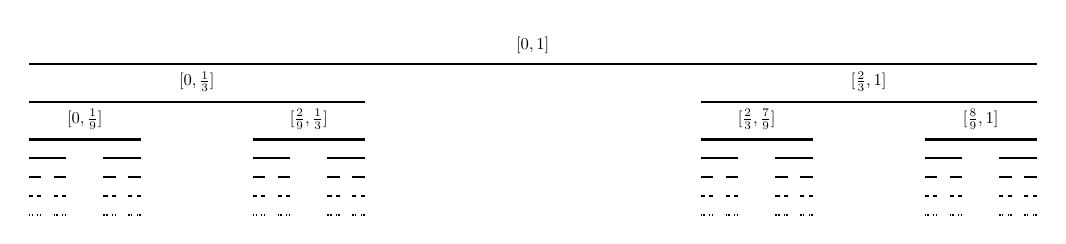
\begin{tikzpicture}[scale=0.8, thick]
      %-------------------------------------------------------------
      % Step 0 (C_0): [0,16], at y = 0
      %-------------------------------------------------------------
      \draw (0,0) -- (16,0)
        node[midway, above] {\scalebox{.6}{$[0,1]$}};
    
      %-------------------------------------------------------------
      % Step 1 (C_1): remove the open middle third (16/3, 32/3) ≈ (5.3333,10.6667)
      % => [0, 5.3333] & [10.6667, 16], at y = -0.6
      %-------------------------------------------------------------
      \draw (0,-0.6) -- (5.3333,-0.6)
        node[midway, above] {\scalebox{.6}{$[0,\frac{1}{3}]$}};
      \draw (10.6667,-0.6) -- (16,-0.6)
        node[midway, above] {\scalebox{.6}{$[\frac{2}{3},1]$}};
    
      %-------------------------------------------------------------
      % Step 2 (C_2): each segment length 5.3333
      % remove its middle third of length ~1.7778
      % => four segments, at y = -1.2
      %-------------------------------------------------------------
      \draw (0,-1.2) -- (1.7778,-1.2)
        node[midway, above] {\scalebox{.6}{$[0,\frac{1}{9}]$}};
      \draw (3.5556,-1.2) -- (5.3333,-1.2)
        node[midway, above] {\scalebox{.6}{$[\frac{2}{9},\frac{1}{3}]$}};
      \draw (10.6667,-1.2) -- (12.4444,-1.2)
        node[midway, above] {\scalebox{.6}{$[\frac{2}{3},\frac{7}{9}]$}};
      \draw (14.2222,-1.2) -- (16,-1.2)
        node[midway, above] {\scalebox{.6}{$[\frac{8}{9},1]$}};
    
      %-------------------------------------------------------------
      % Step 3 (C_3): each segment length ~1.7778
      % remove middle third ~0.5926
      % => 8 segments, at y = -1.5
      %-------------------------------------------------------------
      \draw (0,-1.5)        -- (0.5926,-1.5);
      \draw (1.1852,-1.5)   -- (1.7778,-1.5);
      \draw (3.5556,-1.5)   -- (4.1482,-1.5);
      \draw (4.7408,-1.5)   -- (5.3333,-1.5);
      \draw (10.6667,-1.5)  -- (11.2593,-1.5);
      \draw (11.8519,-1.5)  -- (12.4444,-1.5);
      \draw (14.2222,-1.5)  -- (14.8148,-1.5);
      \draw (15.4074,-1.5)  -- (16,-1.5);
    
      %=============================================================
      % Step 4 (unlabeled), at y = -1.8  (was -2.1 previously)
      % Each segment is length ~0.5926.
      % Remove the middle third (~0.1975).
      %=============================================================
      % From [0, 0.5926]
      \draw (0,-1.8)        -- (0.1975,-1.8);
      \draw (0.3951,-1.8)   -- (0.5926,-1.8);
    
      % From [1.1852,1.7778]
      \draw (1.1852,-1.8)   -- (1.3827,-1.8);
      \draw (1.5802,-1.8)   -- (1.7778,-1.8);
    
      % From [3.5556,4.1482]
      \draw (3.5556,-1.8)   -- (3.7531,-1.8);
      \draw (3.9506,-1.8)   -- (4.1482,-1.8);
    
      % From [4.7408,5.3333]
      \draw (4.7408,-1.8)   -- (4.9383,-1.8);
      \draw (5.1358,-1.8)   -- (5.3333,-1.8);
    
      % From [10.6667,11.2593]
      \draw (10.6667,-1.8)  -- (10.8642,-1.8);
      \draw (11.0617,-1.8)  -- (11.2593,-1.8);
    
      % From [11.8519,12.4444]
      \draw (11.8519,-1.8)  -- (12.0494,-1.8);
      \draw (12.2469,-1.8)  -- (12.4444,-1.8);
    
      % From [14.2222,14.8148]
      \draw (14.2222,-1.8)  -- (14.4197,-1.8);
      \draw (14.6172,-1.8)  -- (14.8148,-1.8);
    
      % From [15.4074,16]
      \draw (15.4074,-1.8)  -- (15.6049,-1.8);
      \draw (15.8024,-1.8)  -- (16,-1.8);
    
      %=============================================================
      % Step 5 (unlabeled), at y = -2.1  (was -3.0 previously)
      % Each segment now length ~0.1975; remove ~0.0658 from middle.
      % So each segment spawns 2 smaller segments.
      %=============================================================
      % From [0.0000, 0.1975]
      \draw (0.0000,-2.1) -- (0.0658,-2.1);
      \draw (0.1317,-2.1) -- (0.1975,-2.1);
    
      % From [0.3951, 0.5926]
      \draw (0.3951,-2.1) -- (0.4609,-2.1);
      \draw (0.5268,-2.1) -- (0.5926,-2.1);
    
      % From [1.1852, 1.3827]
      \draw (1.1852,-2.1) -- (1.2510,-2.1);
      \draw (1.3169,-2.1) -- (1.3827,-2.1);
    
      % From [1.5802,1.7778]
      \draw (1.5802,-2.1) -- (1.6460,-2.1);
      \draw (1.7119,-2.1) -- (1.7778,-2.1);
    
      % From [3.5556,3.7531]
      \draw (3.5556,-2.1) -- (3.6214,-2.1);
      \draw (3.6873,-2.1) -- (3.7531,-2.1);
    
      % From [3.9506,4.1482]
      \draw (3.9506,-2.1) -- (4.0164,-2.1);
      \draw (4.0823,-2.1) -- (4.1482,-2.1);
    
      % From [4.7408,4.9383]
      \draw (4.7408,-2.1) -- (4.8066,-2.1);
      \draw (4.8725,-2.1) -- (4.9383,-2.1);
    
      % From [5.1358,5.3333]
      \draw (5.1358,-2.1) -- (5.2016,-2.1);
      \draw (5.2675,-2.1) -- (5.3333,-2.1);
    
      % From [10.6667,10.8642]
      \draw (10.6667,-2.1) -- (10.7325,-2.1);
      \draw (10.7984,-2.1) -- (10.8642,-2.1);
    
      % From [11.0617,11.2593]
      \draw (11.0617,-2.1) -- (11.1275,-2.1);
      \draw (11.1934,-2.1) -- (11.2593,-2.1);
    
      % From [11.8519,12.0494]
      \draw (11.8519,-2.1) -- (11.9177,-2.1);
      \draw (11.9836,-2.1) -- (12.0494,-2.1);
    
      % From [12.2469,12.4444]
      \draw (12.2469,-2.1) -- (12.3127,-2.1);
      \draw (12.3786,-2.1) -- (12.4444,-2.1);
    
      % From [14.2222,14.4197]
      \draw (14.2222,-2.1) -- (14.2880,-2.1);
      \draw (14.3539,-2.1) -- (14.4197,-2.1);
    
      % From [14.6172,14.8148]
      \draw (14.6172,-2.1) -- (14.6830,-2.1);
      \draw (14.7489,-2.1) -- (14.8148,-2.1);
    
      % From [15.4074,15.6049]
      \draw (15.4074,-2.1) -- (15.4732,-2.1);
      \draw (15.5391,-2.1) -- (15.6049,-2.1);
    
      % From [15.8024,16.0000]
      \draw (15.8024,-2.1) -- (15.8682,-2.1);
      \draw (15.9341,-2.1) -- (16.0000,-2.1);
    
      %=============================================================
      % Step 6 (unlabeled), at y = -2.4
      % Each segment in Step 5 is ~0.0658 in length,
      % remove the middle third (~0.0219).
      % => 64 segments total
      %=============================================================
      % [a, b] => [a, a+0.0219], [a+0.0439, b]
      % 
      % 1) [0.0000, 0.0658]
      \draw (0.0000,-2.4) -- (0.0219,-2.4);
      \draw (0.0439,-2.4) -- (0.0658,-2.4);
    
      % 2) [0.1317, 0.1975]
      \draw (0.1317,-2.4) -- (0.1536,-2.4);
      \draw (0.1756,-2.4) -- (0.1975,-2.4);
    
      % 3) [0.3951, 0.4609]
      \draw (0.3951,-2.4) -- (0.4170,-2.4);
      \draw (0.4390,-2.4) -- (0.4609,-2.4);
    
      % 4) [0.5268, 0.5926]
      \draw (0.5268,-2.4) -- (0.5487,-2.4);
      \draw (0.5707,-2.4) -- (0.5926,-2.4);
    
      % 5) [1.1852, 1.2510]
      \draw (1.1852,-2.4) -- (1.2071,-2.4);
      \draw (1.2291,-2.4) -- (1.2510,-2.4);
    
      % 6) [1.3169, 1.3827]
      \draw (1.3169,-2.4) -- (1.3388,-2.4);
      \draw (1.3608,-2.4) -- (1.3827,-2.4);
    
      % 7) [1.5802, 1.6460]
      \draw (1.5802,-2.4) -- (1.6021,-2.4);
      \draw (1.6241,-2.4) -- (1.6460,-2.4);
    
      % 8) [1.7119, 1.7778]
      \draw (1.7119,-2.4) -- (1.7338,-2.4);
      \draw (1.7558,-2.4) -- (1.7778,-2.4);
    
      % 9) [3.5556, 3.6214]
      \draw (3.5556,-2.4) -- (3.5775,-2.4);
      \draw (3.5995,-2.4) -- (3.6214,-2.4);
    
      % 10) [3.6873, 3.7531]
      \draw (3.6873,-2.4) -- (3.7092,-2.4);
      \draw (3.7312,-2.4) -- (3.7531,-2.4);
    
      % 11) [3.9506, 4.0164]
      \draw (3.9506,-2.4) -- (3.9725,-2.4);
      \draw (3.9945,-2.4) -- (4.0164,-2.4);
    
      % 12) [4.0823, 4.1482]
      \draw (4.0823,-2.4) -- (4.1042,-2.4);
      \draw (4.1262,-2.4) -- (4.1482,-2.4);
    
      % 13) [4.7408, 4.8066]
      \draw (4.7408,-2.4) -- (4.7627,-2.4);
      \draw (4.7847,-2.4) -- (4.8066,-2.4);
    
      % 14) [4.8725, 4.9383]
      \draw (4.8725,-2.4) -- (4.8944,-2.4);
      \draw (4.9164,-2.4) -- (4.9383,-2.4);
    
      % 15) [5.1358, 5.2016]
      \draw (5.1358,-2.4) -- (5.1577,-2.4);
      \draw (5.1797,-2.4) -- (5.2016,-2.4);
    
      % 16) [5.2675, 5.3333]
      \draw (5.2675,-2.4) -- (5.2894,-2.4);
      \draw (5.3114,-2.4) -- (5.3333,-2.4);
    
      % 17) [10.6667, 10.7325]
      \draw (10.6667,-2.4) -- (10.6886,-2.4);
      \draw (10.7106,-2.4) -- (10.7325,-2.4);
    
      % 18) [10.7984, 10.8642]
      \draw (10.7984,-2.4) -- (10.8203,-2.4);
      \draw (10.8423,-2.4) -- (10.8642,-2.4);
    
      % 19) [11.0617, 11.1275]
      \draw (11.0617,-2.4) -- (11.0836,-2.4);
      \draw (11.1056,-2.4) -- (11.1275,-2.4);
    
      % 20) [11.1934, 11.2593]
      \draw (11.1934,-2.4) -- (11.2153,-2.4);
      \draw (11.2373,-2.4) -- (11.2593,-2.4);
    
      % 21) [11.8519, 11.9177]
      \draw (11.8519,-2.4) -- (11.8738,-2.4);
      \draw (11.8958,-2.4) -- (11.9177,-2.4);
    
      % 22) [11.9836, 12.0494]
      \draw (11.9836,-2.4) -- (12.0055,-2.4);
      \draw (12.0275,-2.4) -- (12.0494,-2.4);
    
      % 23) [12.2469, 12.3127]
      \draw (12.2469,-2.4) -- (12.2688,-2.4);
      \draw (12.2908,-2.4) -- (12.3127,-2.4);
    
      % 24) [12.3786, 12.4444]
      \draw (12.3786,-2.4) -- (12.4005,-2.4);
      \draw (12.4225,-2.4) -- (12.4444,-2.4);
    
      % 25) [14.2222, 14.2880]
      \draw (14.2222,-2.4) -- (14.2441,-2.4);
      \draw (14.2661,-2.4) -- (14.2880,-2.4);
    
      % 26) [14.3539, 14.4197]
      \draw (14.3539,-2.4) -- (14.3758,-2.4);
      \draw (14.3978,-2.4) -- (14.4197,-2.4);
    
      % 27) [14.6172, 14.6830]
      \draw (14.6172,-2.4) -- (14.6391,-2.4);
      \draw (14.6611,-2.4) -- (14.6830,-2.4);
    
      % 28) [14.7489, 14.8148]
      \draw (14.7489,-2.4) -- (14.7708,-2.4);
      \draw (14.7928,-2.4) -- (14.8148,-2.4);
    
      % 29) [15.4074, 15.4732]
      \draw (15.4074,-2.4) -- (15.4293,-2.4);
      \draw (15.4513,-2.4) -- (15.4732,-2.4);
    
      % 30) [15.5391, 15.6049]
      \draw (15.5391,-2.4) -- (15.5610,-2.4);
      \draw (15.5830,-2.4) -- (15.6049,-2.4);
    
      % 31) [15.8024, 15.8682]
      \draw (15.8024,-2.4) -- (15.8243,-2.4);
      \draw (15.8463,-2.4) -- (15.8682,-2.4);
    
      % 32) [15.9341, 16.0000]
      \draw (15.9341,-2.4) -- (15.9560,-2.4);
      \draw (15.9780,-2.4) -- (16.0000,-2.4);
    
    \end{tikzpicture}
    \end{center}
    \vspace{35pt}

    We are interested in studying the topological properties of the points which are not deleted at any step of this infinite process. The set of these points have a special name and are defined below.

    \begin{definition}
        Let $C_0 := [0,1]$ and $C_n = \frac{C_{n-1}}{3} \cup \left( \frac{2}{3} + \frac{C_{n-1}}{3}\right)$ for $n \geq 1$. The \textit{Cantor set} is $\fC = \bigcap_{n = 0}^\infty C_n$.
    \end{definition}

    \begin{proposition}
        The Cantor set is closed.
    \end{proposition}
        \begin{proof}
            Since the Cantor set is defined as the intersection of closed sets, it must be closed.
        \end{proof}

    \begin{proposition}
        The Cantor set is nowhere dense.
    \end{proposition}
        \begin{proof}
            Suppose towards contradiction its not, that is, $\overline{\fC}^o \neq \emptyset$. Then there is some $x \in \overline{\fC}^o$. We can find an $\epsilon > 0$ with $(x- \epsilon, x+\epsilon) \subseteq \fC$, in particular $(x- \epsilon, x+\epsilon) \subseteq C_n$ for all $n \geq 1$. Find $m$ large so that $\epsilon > \frac{1}{3^m}$ and consider $(x-\epsilon,x+\epsilon) \subseteq C_m$. We have that $C_m = \bigsqcup_{j = 1}^{2^m}C_{m,j}$ where $\text{length}(C_{m,j}) = \frac{1}{3^m}$. Since each $C_{m,j}$ is disjoint, it must be the case that $(x-\epsilon,x+\epsilon) \subseteq C_{m,j}$ for some $1 \leq j \leq 2^m$. But the length of $(x-\epsilon,x+\epsilon)$ is $2\epsilon$, which is impossible. It must be that $\fC$ is nowhere dense.
        \end{proof}
    
    \begin{proposition}
        The total length of the Cantor set is $0$.
    \end{proposition}
        \begin{proof}
            The total length of the removed intervals is:
                \begin{equation*}
                \begin{split}
                    \frac{1}{3} + \frac{2}{9} + \frac{4}{27} + ... 
                    & = \sum_{k=1}^\infty \frac{2^{k-1}}{3^k} \\
                    & = \frac{1}{2} \sum_{k=1}^\infty \left( \frac{2}{3} \right)^k \\
                    & = \frac{1}{2} \cdot \frac{\sfrac{2}{3}}{1 - \sfrac{2}{3}} \\
                    & = 1.
                \end{split}
                \end{equation*}
            Thus $\text{length}(\fC) = 0$.
        \end{proof}

    \begin{lemma}***
        
    \end{lemma}
        \begin{proof}
            
        \end{proof}

    \begin{lemma}***
    
    \end{lemma}
        \begin{proof}
            
        \end{proof}

    \begin{lemma}***

    \end{lemma}
        \begin{proof}
            
        \end{proof}

    \begin{proposition}***
        $\card(\fC) = \fc$.
    \end{proposition}
        \begin{proof}
            
        \end{proof}

\section{Convergent Sequences}
    \begin{definition}
        Fix a metric space $(X,d)$.
        \begin{enumerate}[label = (\arabic*),itemsep=1pt,topsep=3pt]
            \item A \textit{sequence} in $X$ is a map $x:\bfN \rightarrow X$ defined by $n \mapsto x_n$. We denote a sequence as $(x_n)_{n \geq 1}$, $(x_n)_{n = 1}^\infty$, or $(x_n)_n$.
            
            \item A \textit{natural sequence} is a sequence $(x_n)_n$ in $\bfN$ with $n_1 < n_2 < n_3 < ...$
            
            \item A \textit{subsequence} of a sequence $(x_n)_n$ is a sequence $(x_{n_k})_k$ where $(n_k)_k$ is a natural sequence. This is equivalent to the composition of maps
                    \begin{tikzcd}
                        \bfN \arrow[r, "k \mapsto n_k"] & \bfN \arrow[r, "n_k \mapsto x_{n_k}"] & X.
                    \end{tikzcd}
        \end{enumerate}
    \end{definition}

    \begin{definition}

        A sequence $(x_n)_n$ \textit{converges} to $x \in X$ if:
            \begin{equation*}
            \begin{split}
                (\forall \epsilon > 0)(\exists N \in \bfN):(\forall n \in \bfN)(n \geq N \implies d(x_n,x) < \epsilon).
            \end{split}
            \end{equation*}
        We write $(x_n)_n \xrightarrow{d} x$ or $\limit x_n = x$.
    \end{definition}

    \begin{exercise}
        Show that a sequence can have at most one limit.
    \end{exercise}

    \begin{proposition}
        Given $(x_n)_n$ in $X$ and $x \in X$, the following are equivalent:
        \begin{enumerate}[label = (\arabic*),itemsep=1pt,topsep=3pt]
            \item $(x_n)_n \rightarrow x$ in $X$;
            \item $(d(x_n,x))_n \rightarrow 0$ in $\bfR$;
            \item $(\forall V \in \cN_x)(\exists N \in \bfN):(\forall n\in \bfN)(n \geq N \implies x_n \in V)$. 
        \end{enumerate}
    \end{proposition}

    \begin{exercise}
        Let $(X,d)$ be a metric space and $\rho(x,y) = \frac{d(x,y)}{1 + d(x,y)}$. Then $(x_n)_n \xrightarrow{d} x$ if and only if $(x_n)_n \xrightarrow{\rho} x$.
    \end{exercise}

    \begin{proposition}
        Convergent sequences are bounded.
    \end{proposition}
        \begin{proof}
            Suppose that $(x_n)_n \rightarrow x$ and let $\epsilon = 1$. Find $N$ large so that for $n \geq N$ we have $d(x_n,x) < 1$. Then for all $m,n \geq N$, we have $d(x_m,x_n) \leq d(x_m,x) + d(x,x_n) < 2$. Set $C = \max_{1 \leq n,m \leq N}d(x_m,x_n)$. Now if $n \geq N$ and $m \leq N$, we have:
                \begin{equation*}
                \begin{split}
                    d(x_n,x_m)
                    & \leq d(x_n,x_N) + d(x_N,x_m) \\
                    & \leq 1 + C.
                \end{split}
                \end{equation*}
            Let $K = \max\{2,1+C,C\}$. Then $\diam(\{x_n\}_{n \geq 1}) = \sup_{m,n \geq 1}d(x_n,x_m) \leq K$.
        \end{proof}

    \begin{center}
        \begin{tikzpicture}
            \draw[thick] (0.3,0) -- (2.3,0);
            \node at (2.39, 0) {$/\,$};
            \node at (2.56, 0) {$/\,$};
            \draw[thick] (2.6,0) -- (4.6,0);
        \end{tikzpicture}
    \end{center}

    \begin{definition}
        Let $(f_n)_n$ be a sequence of functions.
        \begin{enumerate}[label = (\arabic*),itemsep=1pt,topsep=3pt]
            \item $(f_n)_n$ converges \textit{pointwise} to $f \in \cF(\Omega,F)$ if:
                \begin{equation*}
                \begin{split}
                    (\forall x \in \Omega)(\forall \epsilon > 0)(\exists N_{x,\epsilon} \in \bfN) : (\forall n \in \bfN)( n \geq N \implies |f_n(x) - f(x)| < \epsilon).
                \end{split}
                \end{equation*}

            \item $(f_n)_n$ converges \textit{uniformly} to $f \in \cF(\Omega,F)$ if:
                \begin{equation*}
                \begin{split}
                        (\forall \epsilon > 0)(\exists N_\epsilon \in \bfN) : (\forall n \in \bfN)(\forall x \in \Omega)(n \geq N &\implies |f_n(x) - f(x)| < \epsilon).
                \end{split}
                \end{equation*}
        \end{enumerate}
    \end{definition}

    \begin{example}
        Recall that a sequence $(f_n)_n$ converges to $f$ in $\Bd(\Omega,Y)$ if:
            \begin{equation*}
            \begin{split}
                (D(f_n,f))_n \rightarrow 0 \h5\text{in $\bfR$}.
            \end{split}
            \end{equation*}
        But this is equivalent to:
            \begin{equation*}
            \begin{split}
                \sup_{x \in \Omega}d(f_n(x),f(x)) \rightarrow 0 \h5\text{in $\bfR$}.
            \end{split}
            \end{equation*}
        Again, we can rewrite this as:
            \begin{equation*}
            \begin{split}
                (\forall \epsilon > 0)(\exists N \in \bfN):(\forall n \in \bfN)\Bigl(n\geq N \implies \sup_{x \in \Omega}d(f_n(x),f(x))<\epsilon\Bigr).
            \end{split}
            \end{equation*}
        But this definition is equivalent to:
            \begin{equation*}
            \begin{split}
                (\forall \epsilon > 0)(\exists N \in \bfN):(\forall n \in \bfN)(\forall x\in \Omega)\Bigl(n\geq N \implies d(f_n(x),f(x))<\epsilon\Bigr).
            \end{split}
            \end{equation*}
        This is precisely the definition of uniform convergence. Thus convergence in $c_{00} \subseteq c_0 \subseteq c \subseteq \ell_\infty \subseteq \ell_\infty(\Omega) = \Bd(\Omega,F)$ is uniform.
    \end{example}

    \begin{proposition}
        Let $(d_k)_k$ be a separating family of semi-metrics which are uniformly bounded. Define:
            \begin{equation*}
            \begin{split}
                d(x,y) := \sum_{k = 1}^\infty 2^{-k}d_k(x,y).
            \end{split}
            \end{equation*}
        Then $(x_n)_n \xrightarrow{d} x$ if and only if for all $k$, $(d_k(x_n,x))_n \rightarrow 0$.
    \end{proposition}
        \begin{proof}
            Fix $k$. We have:
                \begin{equation*}
                \begin{split}
                    0 \leq 2^{-k}d_k(x_n,x) \leq d(x_n,x).
                \end{split}
                \end{equation*}
            Note that $(x_n)_n \xrightarrow{d} x$ implies $(d(x_n,x))_n \rightarrow 0$. Multiplying both sides of the above equation by $2^k$ and applying the squeeze theorem gives $(d_k(x_n,x)) \rightarrow 0$.

            Now let $\epsilon > 0$. Since each $d_k$ is uniformly bounded, let $C = \sup_{k,x,y}d(x,y)$. Find $K$ large so that:
                \begin{equation*}
                \begin{split}
                    \sum_{k > K}2^{-k} < \frac{\epsilon}{2C}.
                \end{split}
                \end{equation*}
            We know $(d_k(x_n,x))_n \rightarrow 0$ for $k = 1,2,...,K$. So there exists $N_1,N_2,...,N_K$ with $n \geq N_k$ implying $d_k(x_n,x) < \frac{\epsilon}{2}$. Let $N = \max_{k = 1}^K N_k$. For $n \geq N$, we have:
                \begin{equation*}
                \begin{split}
                    d(x_n,x) 
                    & = \sum_{k = 1}^K 2^{-k}d_k(x_n,x) + \sum_{k > K}2^{-k}d_k(x_n,x) \\
                    & = \sum_{k = 1}^K 2^{-k}d_k(x_n,x) + \sum_{k > K}2^{-k} C \\
                    & < \sum_{k = 1}^K 2^{-k} \frac{\epsilon}{2} + C \cdot \frac{\epsilon}{2C} \\
                    & \leq \frac{\epsilon}{2} + \frac{\epsilon}{2} \\
                    & = \epsilon. \qedhere
                \end{split}
                \end{equation*}
        \end{proof}

    \begin{example}
        Let $X = C(\bfR)$. How does one define a distance between two functions on this space? For $f,g \in C(\bfR)$, one might naively consider the uniform metric:
            \begin{equation*}
            \begin{split}
                d(f,g) := \sup_{x \in \Omega}|f(x) - g(x)|.
            \end{split}
            \end{equation*}
        This construction does not guarantee $d(f,g) < \infty$. We can fix this as follows\textemdash for each $k \geq 1$, let:
            \begin{equation*}
            \begin{split}
                P_k(f) = \sup_{x \in [-k,k]}|f(x)|.
            \end{split}
            \end{equation*}
        Then $\{P_k\}_k = 1^\infty$ is a separating family of semi-norms which generate a separating family of semi-metrics:
            \begin{equation*}
            \begin{split}
                \rho_k(f,g) := P_k(f-g).
            \end{split}
            \end{equation*}
        These are not uniformly bounded, so make:
            \begin{equation*}
            \begin{split}
                d_k(f,g) = \frac{\rho_k(f,g)}{1 + \rho_k(f,g)}.
            \end{split}
            \end{equation*}
        Then $\{d_k\}_{k=1}^\infty$ is a family of uniformly bounded semi-metrics. We can now define the \textit{Fr\'echet metric}:
            \begin{equation*}
            \begin{split}
                d_F(f,g) := \sum_{k = 1}^\infty 2^{-k}d_k(f,g).
            \end{split}
            \end{equation*}
        In $(C(\bfR),d_F)$, observe that:
            \begin{equation*}
            \begin{split}
                (f_n)_n \xrightarrow{d_F}f 
                &\iff \forall k, (d_k(f_n,f))_n \rightarrow 0 \\
                &\iff \forall k, (\rho_k(f_n,f))_n \rightarrow 0 \\
                &\iff \forall k, \Bigl(\ts \sup_{x \in [-k,k]}|f_n(x) - f(x)|\Bigr)_n \rightarrow 0 \\
                &\iff \forall k, (f_n)_n \rightarrow f \h5\text{uniformly on $[-k,k]$}.
            \end{split}
            \end{equation*}
        We've obtained a new type of convergence defined below.
    \end{example}

    \begin{definition}
        Let $(X,\tau)$ be a topological space and $(Y,d_Y)$ be a metric space. A sequence of functions:
            \begin{equation*}
            \begin{split}
                f_n:X \rightarrow Y; \h5 n \in \bfN
            \end{split}
            \end{equation*}
        converges \textit{compactly} to $f:X \rightarrow Y$ if, for every compact set $K \subseteq X$, the sequence $\left( \restr{f_n}{K} \right)_n \rightarrow \restr{f}{K}$ converges uniformly.
    \end{definition}

    \begin{example}***
        $x^n$ does not converge uniformly but it does converge compactly (idk how to do this)
    \end{example}

    \begin{center}
        \begin{tikzpicture}
            \draw[thick] (0.3,0) -- (2.3,0);
            \node at (2.39, 0) {$/\,$};
            \node at (2.56, 0) {$/\,$};
            \draw[thick] (2.6,0) -- (4.6,0);
        \end{tikzpicture}
    \end{center}

    \begin{example}
        Let $(X,d)$, $(Y,\rho)$ be metric spaces. There are different metrics we may put on $X \times Y$, for example:
            \begin{itemize}
                \item $D_1((x,y),(x',y')) = d(x,x') + \rho(y,y')$ 
                \item $D_2((x,y),(x',y')) = \sqrt{d(x,x')^2 + \rho(y,y')^2}$
                \item $D_\infty((x,y),(x',y')) = \max\{d(x,x') + \rho(y,y')\}$.
            \end{itemize}
        These metrics are all equivalent. A sequence of points $(x_n,y_n)_n$ converges to $(x,y)$ in $X \times Y$ with respect to any of these metrics if and only if $(x_n)_n \xrightarrow{d} x$ and $(y_n)_n \xrightarrow{\rho} y$.
    \end{example}

    \begin{example}
        Let $\{(X_k,d_k)_k\}_k$ be a family of metric spaces where the $d_k$ are uniformly bounded. We looked at the product:
            \begin{equation*}
            \begin{split}
                X = \prod_{k = 1}^\infty X_k
            \end{split}
            \end{equation*}
        with:
            \begin{equation*}
            \begin{split}
                d(f,g) = \sum_{k = 1}^\infty 2^{-k}d_k(f(k),g(k)).
            \end{split}
            \end{equation*}
        We have that $(f_n)_n \xrightarrow{d} f$ if and only if $(f_n(k))_n \rightarrow f(k)$ for all $k$ (pointwise convergence).
    \end{example}

    \begin{example}
        Let $(V,\lnorm \cdot \rnorm)$ be a normed space. Then $(v_n)_n \rightarrow v$ if and only if $(\lnorm v_n - v \rnorm)_n \rightarrow 0$.
    \end{example}

    \begin{definition}
        Let $(v_k)_k$ be a sequence in $(V,\lnorm \cdot \rnorm)$.
        \begin{enumerate}[label = (\arabic*),itemsep=1pt,topsep=3pt]
            \item A \textit{sequence of partial sums} $(s_n)_n$ is defined as $s_n = \sum_{k = 1}^n v_k$.
            \item If $(s_n)_n \rightarrow s$ in $V$ we say the \textit{series} $\sum_{k = 1}^\infty v_k$ converges and write $\sum_{k = 1}^\infty v_k = s$.
            \item The series $\sum v_k$ converges \textit{absolutely} if $\sum \lnorm v_k \rnorm$ converges.
        \end{enumerate}
    \end{definition}

    \begin{center}
        \begin{tikzpicture}
            \draw[thick] (0.3,0) -- (2.3,0);
            \node at (2.39, 0) {$/\,$};
            \node at (2.56, 0) {$/\,$};
            \draw[thick] (2.6,0) -- (4.6,0);
        \end{tikzpicture}
    \end{center}

    \begin{proposition}\label{prop:1}
        Let $(X,d)$ be a metric space and $A \subseteq X$. We have $x \in \overline{A}$ if and only if there exists a sequence $(a_n)_n$ in $A$ with $(a_n)_n \rightarrow x$.
    \end{proposition}
        \begin{proof}
            Let $x \in \overline{A}$. For each $n \geq 1$, we have $U(x,\frac{1}{n}) \cap A \neq \emptyset$, so choose $a_n \in U(x,\frac{1}{n}) \cap A$. Then $d(x,a_n) < \frac{1}{n}$, so $(a_n)_n \rightarrow x$.

            Now suppose $(a_n)_n$ is a sequence in $A$ and $(a_n)_n \rightarrow x$. Given $\epsilon > 0$, find $N$ large so $d(x,a_N) < \epsilon$. Then $a_N \in U(x,\epsilon) \cap A$. Since $U(x,\epsilon) \cap A \neq \emptyset$, we have $x \in \overline{A}$. 
        \end{proof}

    \begin{proposition}\label{prop:closed-iff-seq}
        Let $(X,d)$ be a metric space and $A \subseteq X$. The following are equivalent:
            \begin{enumerate}[label = (\arabic*),itemsep=1pt,topsep=3pt]
                \item $A$ is closed;
                \item If $(a_n)_n$ is a sequence in $A$ which converges to $x \in X$, then $x \in A$.
            \end{enumerate}
    \end{proposition}
        \begin{proof}
            Consider the sequence $(a_n)_n$ in $A$ with $(a_n)_n \rightarrow x$. Then by the previous proposition $x \in \overline{A}$. But since $A$ is closed, $A = \overline{A}$. Thus $x \in A$.

            To show $A$ is closed we show $A = \overline{A}$. Clearly $A \subseteq \overline{A}$. Let $x \in \overline{A}$. Then there exists a sequence $(a_n)_n$ in $A$ with $(a_n)_n \rightarrow x$. So $x \in A$ by (2). Thus $\overline{A} \subseteq A$.
        \end{proof}

    \begin{exercise}
        Show $x \in \overline{A}$ if and only if $x \in A$ or there exists a sequence $(a_n)_n$ in $A \setminus\{a\}$ with $(a_n)_n \rightarrow x$.
    \end{exercise}

    \begin{example}***
        The space $c_0 \subseteq \ell_\infty$ is closed, and furthermore $\overline{c_{00}} = c_0$. To see this, consider a sequence $(z_n)_n$ in $c_0$ converging to $f \in \ell_\infty$. We will show that $f \in c_0$.

        Let $\epsilon > 0$ be given. Find $N$ large so that:
            \begin{equation*}
            \begin{split}
                \lnorm z_N - f \rnorm_u < \frac{\epsilon}{2}.
            \end{split}
            \end{equation*}
        Since $z_N \in c_0$, we know $\lim_{k \rightarrow \infty}z_N(k) = 0$. So find $K$ large so that for $k \geq K$:
            \begin{equation*}
            \begin{split}
                |z_N(k)| < \frac{\epsilon}{2}.
            \end{split}
            \end{equation*}
        Putting this all together, for $k \geq K$ we have:
            \begin{equation*}
            \begin{split}
                |f(k)|
                & = |f(k) - z_N(k) + z_N(k)| \\
                & \leq |f(k) - z_N(k)| + |z_N(k)| \\
                & < \frac{\epsilon}{2} + \frac{\epsilon}{2} \\
                & = \epsilon.
            \end{split}
            \end{equation*}
        Thus $f \in c_0$. By Proposition~\ref{prop:closed-iff-seq}, $c_0$ is closed.
    \end{example}

    \begin{definition}
        Let $(X,d)$ be a metric space and $A \subseteq X$. The \textit{distance} of an element $x \in X$ to $A$ is a map $\text{dist}_A:X \rightarrow [0,\infty)$ defined by $\text{dist}_A(x) = \inf_{a \in A}d(x,a)$.
    \end{definition}

    \begin{proposition}***
        
    \end{proposition}

\section{Continuity}
    \begin{definition}\label{def:2.5}
        Let $(X,d)$ and $(Y,\rho)$ be metric spaces. A map $f:X \rightarrow Y$ is \textit{continuous at $x_0 \in X$} if any of the equivalent definitions are satisfied:
            \begin{enumerate}[label = (\arabic*),itemsep=1pt,topsep=3pt]
                \item $(\forall \epsilon > 0)(\exists \delta > 0):(\forall x \in X)\Bigl(d(x,x_0) < \delta \implies \rho\bigl(f(x),f(x_0)\bigr) < \epsilon\Bigr)$
                \item $(\forall \epsilon > 0)(\exists \delta > 0):(\forall x \in X)\Bigl(x \in U_X(x_0, \delta) \implies f(x) \in U_Y\bigl(f(x_0),\epsilon\bigr)\Bigr)$
                \item $(\forall \epsilon > 0)(\exists \delta > 0):f\bigl(U_X(x_0,\delta)\bigr) \subseteq U_Y\bigl(f(x_0),\epsilon\bigr)$
            \end{enumerate}
    \end{definition}

    \begin{proposition}
        Let $f:(X,d) \rightarrow (Y,\rho)$ be a map between metric spaces and $x_0 \in X$. The following are equivalent:
            \begin{enumerate}[label = (\arabic*),itemsep=1pt,topsep=3pt]
                \item $f$ is continuous at $x_0$;
                \item $(\forall V \in \cN_{f(x_0)})(\exists U \in \cN_{x_0}):f(U) \subseteq V$;
                \item $(\forall (x_n)_n \in X^\bfN)\bigl((x_n)_n \rightarrow x_0 \implies (f(x_n))_n \rightarrow f(x_0)\bigr)$
            \end{enumerate}
    \end{proposition}
        \begin{proof}
            (1)$\Rightarrow$(2) follows from Definition~\ref{def:2.5}. 
            
            (1)$\Rightarrow$(3) Let $(x_n)_n \rightarrow x_0$. Let $\epsilon > 0$. Since $f$ is continuous, find $\epsilon > 0$ do that $x \in U(x,\delta)$ implies $f(x) \in U(f(x_0),\epsilon)$. Whence $d(f(x_n),f(x_0)) < \epsilon$, establishing $(f(x_n))_n \rightarrow f(x_0)$.

            (3)$\Rightarrow$(1) We prove the contrapositive of this statement. If $f$ is not continuous, choose $\epsilon_0>0$ so that $d(x_n,x_0) < \frac{1}{n}$ and $d(f(x_n),f(x_0)) \geq \epsilon_0$. Whence $(x_n)_n \rightarrow x_0$ and $(f(x_n))_n \not\rightarrow f(x_0)$.
        \end{proof}

    \begin{proposition}
        Let $f:(X,d) \rightarrow (Y,\rho)$ be a map of metric spaces. The following are equivalent:
            \begin{enumerate}[label = (\arabic*),itemsep=1pt,topsep=3pt]
                \item $f$ is continuous;
                \item $(\forall V \in \tau_Y),f^{-1}(V) \in \tau_X$;
            \end{enumerate}
    \end{proposition}
        \begin{proof}
            Let $V \subseteq Y$ be open. If $f^{-1}(V) = \emptyset$, we're done. If not, let $x \in f^{-1}(V)$. Then $f(x) \in V$. Since $V$ is open, find $\epsilon > 0$ so that $U(f(x),\epsilon) \subseteq V$. Since $f$ is continuous, find $\delta > 0$ so that $f(U(x,\delta)) \subseteq U(f(x),\epsilon) \subseteq V$. Whence $U(x,\delta) \subseteq f^{-1}(V)$.

            Let $x \in X$ and $\epsilon > 0$. Since $U(f(x),\epsilon) \in \tau_Y$, we have $f^{-1}(U(f(x)),\epsilon) \in \tau_X$. Note that $x \in f^{-1}(U(f(x)),\epsilon)$. Since this set is open, find $\delta > 0$ so that $U(x,\delta) \subseteq f^{-1}(U(f(x)),\epsilon)$. Thus $f(U(x,\delta)) \subseteq U(f(x),\epsilon)$; i.e., $f$ is continuous.
        \end{proof}

    \begin{proposition}
        Let $(X,d) \xrightarrow{f} (Y,\rho) \xrightarrow{g} (Z,\gamma)$ be maps of metric spaces. If $f$ is continuous at $x \in X$ and $g$ is continuous at $y = f(x)$, then $g \circ f$ is continuous at $x$.
    \end{proposition}
        \begin{proof}
            Exercise.
        \end{proof}

    \begin{proposition}
        Let $(X,d)$ be a metric space with $A \subseteq X$ dense. Let $f:X \rightarrow F$ be a continuous and bounded function. Then $\sup_{x \in A}f(x) = \sup_{x \in X}f(x)$.
    \end{proposition}
        \begin{proof}
            Since $A \subseteq X$ we have $\sup_{x \in A}f(x) \leq \sup_{x \in X}f(x)$. Conversely, let $\epsilon > 0$. Find $x' \in X$ so that $\sup_{x \in X}f(x) - \frac{\epsilon}{2} < f(x')$. Since $f$ is continuous, find $\delta > 0$ so that for all $x \in X$, $d(x,x') < \delta$ implies $|f(x)-f(x')| < \frac{\epsilon}{2}$. Since $A$ is dense, find $a \in A$ so that $d(x',a) < \delta$. This implies $|f(x')-f(a)| < \frac{\epsilon}{2}$, or equivalently $f(x')- \frac{\epsilon}{2} < f(a)$. This gives:
                \begin{equation*}
                \begin{split}
                    \sup_{x \in X}f(x) - \epsilon 
                    & < f(a).
                \end{split}
                \end{equation*}
            Hence for $\epsilon > 0$ we have:
                \begin{equation*}
                \begin{split}
                    \sup_{x \in X}f(x)< \sup_{x \in A}f(x) + \epsilon.
                \end{split}
                \end{equation*}
            Taking $\epsilon \rightarrow 0$ gives $\sup_{x \in X}f(x) \leq \sup_{x \in A}f(x)$.
        \end{proof}

    \begin{definition}
        Let $f:(X,d) \rightarrow (Y,\rho)$ be a map of metric spaces.
        \begin{enumerate}[label = (\arabic*),itemsep=1pt,topsep=3pt]
            \item $f$ is \textit{uniformly continuous} if:
                \begin{equation*}
                \begin{split}
                    (\forall \epsilon > 0)(\exists \delta > 0): (\forall x,x' \in X)(d(x,x') < \delta \implies \rho(f(x),f(x')) < \epsilon).
                \end{split}
                \end{equation*}
            \item $f$ is \textit{Lipschitz} if there exists $C > 0$ such that:
                \begin{equation*}
                \begin{split}
                    (\forall x,x' \in X)(\rho(f(x),f(x')) \leq C d(x,x')).
                \end{split}
                \end{equation*}
            If $C < 1$, we say $f$ is \textit{contractive}.

            \item $f$ is \textit{isometric} (or an \textit{isometry}) if:
                \begin{equation*}
                \begin{split}
                    (\forall x,x' \in X)(\rho(f(x),f(x')) = d(x,x'))
                \end{split}
                \end{equation*}
        \end{enumerate}
    \end{definition}

    \begin{exercise}
        Show that Lipschitz implies uniform continuity. Show that uniform continuity implies continuity. Show that the converse direction fails in general.
    \end{exercise}

    \begin{example}
        Let $(V, \lnorm \cdot \rnorm)$ be a normed space. Then $V \xrightarrow{\lnorm \cdot \rnorm} [0,\infty)$ is continuous. Indeed, we have $\left| \lnorm v \rnorm - \lnorm w \rnorm \right| \leq \lnorm v - w \rnorm$, so $\lnorm \cdot \rnorm$ is Lipschitz.
    \end{example}

    \begin{example}
        Let $(X,d)$ be a metric space and equip $X \times X$ with the product metric $D_1$. Claim: $d:X \times X \rightarrow [0,\infty)$ is continuous. Indeed, given $(x,y),(x',y') \in X \times X$, then we have:
            \begin{equation*}
            \begin{split}
                d(x,y) \leq d(x,x') + d(x',y') + d(y',y).
            \end{split}
            \end{equation*}
        So we have $d(x,y) - d(x',y') \leq d(x,x') + d(y,y')$. But this is equivalent to $|d(x,y) - d(x',y')| \leq D_1((x,y),(x',y'))$. So $d$ is Lipschitz.
    \end{example}

    \begin{example}
        If $(X,d)$ is a metric space and $A \subseteq X$, then $\dist_A : X \rightarrow [0,\infty)$ is continuous. We've shown that $|\dist_A(x) - \dist_A(y)| \leq d(x,y)$, so $\dist_A$ is Lipschitz.
    \end{example}

    \begin{definition}
        Let $X$ be a topological space. We say $X$ is \textit{normal} (or T4) if, for any $A,B \subseteq X$ closed satisfying $A \cap B = \emptyset$, then there exists $U,V \in \tau_X$ with $A \subseteq U$, $B \subseteq V$ satisfying $U \cap V = \emptyset$.
    \end{definition}

    \begin{proposition}
        Metric spaces are normal.
    \end{proposition}
        \begin{proof}
            Let $A,B \subseteq (X,d)$ with $A \cap B = \emptyset$. Define $f:(X,d) \rightarrow \bfR$ by:
                \begin{equation*}
                \begin{split}
                    f(x) = \frac{\dist_A(x)}{\dist_A(x) + \dist_B(x)}.
                \end{split}
                \end{equation*}
            Then $f$ is continuous. Moreover, define:
                \begin{equation*}
                \begin{split}
                    U &:= f^{-1}\left(\left(-\sfrac{1}{2},\sfrac{1}{2}\right)\right) \\
                    V &:= f^{-1}\left(\left(-\sfrac{1}{2},\sfrac{3}{2}\right)\right)
                \end{split}
                \end{equation*}
            Then $U$ and $V$ open with $U \cap V = \emptyset$.
        \end{proof}

    \begin{proposition}
        Let $V$ and $W$ be normed spaces and $T:V \rightarrow W$ linear. The following are equivalent:
            \begin{enumerate}[label = (\arabic*),itemsep=1pt,topsep=3pt]
                \item $T$ is continuous at $0_V$;
                \item $T$ is continuous;
                \item $T$ is uniformly continuous;
                \item $T$ is Lipschitz;
                \item there exists $C \geq 0$ such that $\lnorm Tv \rnorm \leq C \lnorm v \rnorm$ for all $v \in V$;
                \item $T$ is bounded.
            \end{enumerate}
    \end{proposition}
        \begin{proof}
            We will show (6)$\Leftrightarrow$(5)$\Rightarrow$(4)$\Rightarrow$(3)$\Rightarrow$(2)$\Rightarrow$(1)$\Rightarrow$(5). Let $T$ be bounded. Given $v \in V$, $v \neq 0$, we have:
                \begin{equation*}
                \begin{split}
                    \lnorm T \rnorm_{\op} 
                    & = \sup_{v \in B_V}\lnorm Tv \rnorm \\
                    & \geq \lnorm T  \frac{v}{\lnorm v \rnorm} \rnorm \h5\text{for all $v \in V$}\\
                    & = \frac{1}{\lnorm v \rnorm} \lnorm Tv \rnorm \h5\text{for all $v \in V$}.
                \end{split}
                \end{equation*}
            Thus $\lnorm Tv \rnorm \leq \lnorm T \rnorm_{\op} \lnorm v \rnorm$ for all $v \in V$. The converse is clear by inspection.

            Suppose there exists $C \geq 0$ satisfying (5). We have that $\lnorm Tv - Tv' \rnorm \leq C \lnorm v - v' \rnorm$. Thus $T$ is Lipschitz.

            Let $T$ be Lipschitz. Let $\epsilon > 0$ and find $\delta = \frac{\epsilon}{c}$. Then $\lnorm v - v' \rnorm < \delta$ implies:
                \begin{equation*}
                \begin{split}
                    \lnorm Tv - Tv' \rnorm
                    & \leq C \lnorm v - v' \rnorm \\
                    & < c \frac{\epsilon}{c} \\
                    & = \epsilon.
                \end{split}
                \end{equation*}
            Thus $T$ is uniformly continuous.

            Suppose that $T$ be uniformly continuous. Fix $x \in V$. Given $\epsilon > 0$, we can find $\delta > 0$ so that $\lnorm v - x \rnorm < \delta$ implies $\lnorm Tv - Tx \rnorm < \epsilon$. Thus $T$ is continuous at $x \in V$. Since $x$ was arbitrary, $T$ is continuous. Moreover, $T$ will be continuous at $0_V$, establishing (1).
            
            We will now show (1) implies (5). Let $\epsilon = 1$. We can find a $\delta > 0$ such that $T\bigl(U(0,\delta)\bigr) \subseteq U(0,1)$. If $v \in V$, $v \neq 0$, then $\frac{\delta v}{2 \lnorm v \rnorm} \in U(0,\delta)$. Since $T$ is continuous at $0$, we have $T\frac{\delta v}{2 \lnorm v \rnorm} \in U(0,1)$\footnote{Recall that $T(0) = 0$.}. This gives $\lnorm T \frac{\delta v}{2 \lnorm v \rnorm} \rnorm < 1$, which is equivalent to $\lnorm Tv \rnorm < \frac{2}{\delta}\lnorm v \rnorm$. This establishes (5).
        \end{proof}

    \begin{corollary}***
        Let $V$ be a normed space and $T:\ell_p^n \rightarrow V$ linear. Then $T$ is uniformly continuous.
    \end{corollary}
        \begin{proof}
            Let $x \in \ell_p^n$ and $\cB = \{e_1,...,e_n\}$ a basis for $\ell_p^n$. Find $\alpha_1,...,\alpha_n$ so that:
                \begin{equation*}
                \begin{split}
                    \lnorm Tv \rnorm
                    & = \lnorm T \left( \sum_{j = 1}^n \alpha_j e_j \right) \rnorm \\
                    & = \lnorm \sum_{j = 1}^n  \alpha_j Te_j\rnorm \\
                    & \leq \sum_{j = 1}^n |\alpha_j| \lnorm T e_j \rnorm \\
                    & \leq c \lnorm \sum_{j = 1}^n \alpha_j e_j \rnorm_1 \\
                    & \leq c \cdot c' \lnorm \sum_{j = 1}^n \alpha_j e_j \rnorm_p,
                \end{split}
                \end{equation*}
            where $c = \max_{j = 1}^n \lnorm Te_j \rnorm$ and $\lnorm \cdot \rnorm_1 \leq c' \lnorm \cdot \rnorm_p$.
        \end{proof}

    \begin{proposition}
        Let $(X,d)$ be a metric space with $A \subseteq X$ dense. If $f,g :X \rightarrow (Y,\rho)$ are continuous with $f(a) = g(a)$ for all $a \in A$, then $f = g$.
    \end{proposition}
        \begin{proof}
            If $x \in X$, we can find a sequence $(a_n)_n$ in $A$ with $(a_n)_n \xrightarrow{d} x$. Then:
                \begin{equation*}
                \begin{split}
                    &(f(a_n))_n \rightarrow f(x) \\
                    & \h9\h3\shortparallel \\
                    & (g(a_n))_n \rightarrow g(x).
                \end{split}
                \end{equation*}
            Thus $f(x) = g(x)$.
        \end{proof}

    \begin{definition}
        Let $(X,d)$ and $(Y,\rho)$ be metric spaces and $f:X \rightarrow Y$.
        \begin{enumerate}[label = (\arabic*),itemsep=1pt,topsep=3pt]
            \item $f$ is a \textit{homeomorphism} if $f$ is bijective with $f$ and $f^{-1}$ continuous. If such an $f$ exists, we say $X \cong Y$ are \textit{homeomorphic}.
            \item $f$ is a \textit{uniformism} if $f$ is bijective with $f$ and $f^{-1}$ uniformly continuous. If such an $f$ exists, we say $X \cong Y$ are \textit{uniformly isomorphic}.
            \item $f$ is an \textit{metric isomorphism} if $f$ is bijective with $f$ and $f^{-1}$ Lipschitz. If such an $f$ exists, we say $X \cong Y$ are \textit{metrically isomorphic}.
            \item $f$ is an \textit{isometric isomorphism} if $f$ and $f^{-1}$ are isometries. We say $X \cong Y$ are \textit{isometrically isomorphic}.
        \end{enumerate}
    \end{definition}

    \begin{example}
        $(0,1) \cong \bfR$ are homeomorphic, but not uniformly isomorphic.
    \end{example}

    \begin{example}***
        Let $a = (a_k)_k \in \ell_1$. Define $\varphi_a:c_0 \rightarrow F$ by $\varphi_a(z) = \sum_{k \geq 1}a_k z_k$. This series converges since:
    \end{example}

    \begin{definition}
        Let $X$ be a set with two metrics $d_1$ and $d_2$.
        \begin{enumerate}[label = (\arabic*),itemsep=1pt,topsep=3pt]
            \item $d_1$ and $d_2$ are \textit{metrically equivalent} if $\id:(X,d_1) \rightarrow (X,d_2)$ and $\id^{-1}:(X,d_2) \rightarrow (X,d_1)$ are Lipschitz.
            \item $d_1$ and $d_2$ are \textit{uniformly equivalent} if $\id:(X,d_1) \rightarrow (X,d_2)$ and $\id^{-1}:(X,d_2) \rightarrow (X,d_1)$ are uniformisms.
            \item $d_1$ and $d_2$ are \textit{topologically equivalent} if $\id:(X,d_1) \rightarrow (X,d_2)$ and $\id^{-1}:(X,d_2) \rightarrow (X,d_1)$ are homeomorphisms.
        \end{enumerate}
    \end{definition}

    \begin{example}***
        
    \end{example}

\section{Completeness}
    \begin{definition}
        A sequence $(x_n)_n$ in a metric space $(X,d)$ is $d$-\textit{Cauchy} if:
            \begin{equation*}
            \begin{split}
                (\forall \epsilon > 0)(\exists N \in \bfN): (\forall p,q \in \bfN)(p,q \geq N \implies d(x_p,x_q) < \epsilon).
            \end{split}
            \end{equation*}
    \end{definition}

    \begin{proposition}
        Let $(x_n)$ be a sequence in $(X,d)$.
        \begin{enumerate}[label = (\arabic*),itemsep=1pt,topsep=3pt]
            \item If $(x_n)_n$ converges, then $(x_n)_n$ is Cauchy.
            \item If $(x_n)_n$ is Cauchy, then $(x_n)_n$ is bounded.
        \end{enumerate}
    \end{proposition}
        \begin{proof}
            (1) Let $x \in X$ and suppose $(x_n)_n \rightarrow x$. Let $\epsilon > 0$. Find $N$ large so that for $p \geq N$ we have $d(x_p,x) < \frac{\epsilon}{2}$. Then $p,q \geq N$ implies:
                \begin{equation*}
                \begin{split}
                    d(x_p,x_q) 
                    & \leq d(x_p,x) + d(x,x_q) \\
                    & < \frac{\epsilon}{2} + \frac{\epsilon}{2} \\
                    & = \epsilon.
                \end{split}
                \end{equation*}

            (2) Let $\epsilon = 1$. Find $N$ large so $p,q \geq N$ implies $d(x_p,x_q) < 1$. Let $C = \max_{1 \leq p,q \leq N}d(x_p,x_q)$. Without loss of generality, if $p \geq N $ and $q \leq N$, then $d(x_p,x_q) \leq d(x_p,x_N) + d(x_N,x_q) < 1 + C$. Set $K = \max\{1,1+C\}$. Then $\diam(\{x_n\}_{n \geq 1}) = \sup_{p,q \geq 1}d(x_p,x_q) < K$.
        \end{proof}

    \begin{proposition}
        Let $(x_n)_n$ be a Cauchy sequence in $X$ and suppose there exists a subsequence $(x_{n_k})_k$ converging to $x \in X$. Then $(x_n)_n$ converges to $x$.
    \end{proposition}
        \begin{proof}
            Let $\epsilon > 0$. Since $(x_n)_n$ is Cauchy, there exists $N$ large so $n,n_k \geq N$ implies $d(x_n,x_{n_k}) < \frac{\epsilon}{2}$. This gives:
                \begin{equation*}
                \begin{split}
                    d(x_n,x) 
                    & = d(x_n,\limit_{k \rightarrow \infty}x_{n_k}) \\
                    & = \limit_{k \rightarrow \infty} d(x_n,x_{n_k}) \\
                    & \leq \frac{\epsilon}{2} \\
                    & < \epsilon. \qedhere
                \end{split}
                \end{equation*}
        \end{proof}

    \begin{definition}
        A metric space is said to be \textit{complete} if every Cauchy sequence converges. A complete normed space is called a \textit{Banach space}. A complete inner product space is called a \textit{Hilbert space}.
    \end{definition}

    \begin{lemma}
        Let $f:(X,d) \rightarrow (Y,\rho)$ be uniformly continuous. If $(x_n)_n$ is $d$-Cauchy then $(f(x_n))_n$ is $\rho$-Cauchy.
    \end{lemma}
        \begin{proof}
            Let $\epsilon > 0$. Find $\delta > 0$ so that $d(x,x') < \delta$ implies $\rho(f(x),f(x')) < \epsilon$. Pick $N$ sufficiently large so that $p,q \geq N$ implies $d(x_p,x_q) < \delta$. This gives $\rho(f(x_p),f(x_q)) < \epsilon$, whence $(f(x_n))_n$ is $\rho$-Cauchy.
        \end{proof}

    \begin{corollary}
        If $f:(X,d) \rightarrow (Y,\rho)$ is a uniformism, then $(X,d)$ is complete if and only if $(Y,\rho)$ is complete.
    \end{corollary}
        \begin{proof}
            Let $(X,d)$ be complete. If $(y_n)_n$ is $\rho$-Cauchy, then $(f^{-1}(y_n))_n$ is $d$-Cauchy in $X$. So we can find some $x \in X$ such that $(f^{-1}(y_n))_n \rightarrow x$. Then $(f(f^{-1}(y_n)))_n = (y_n)_n \rightarrow f(x)$. The converse follows similarly.
        \end{proof}

    \begin{corollary}
        If $d_1$ and $d_2$ are uniformly equivalent metrics on a set $X$, then $(X,d_1)$ is complete if and only if $(X,d_2)$ is complete.
    \end{corollary}
        \begin{proof}
            Since the map $\id:(X,d_1) \rightarrow (X,d_2)$ is a uniformism, the previous corollary gives that $(X,d_1)$ is complete if and only if $(X,d_2)$ is complete.
        \end{proof}
    

    \begin{proposition} 
        $\ell_p^d$ is a Banach space for $1 \leq p \leq \infty$.
    \end{proposition}
        \begin{proof}
            We only need to show this for $\ell_\infty^d$ since all the $p$-norms are equivalent. Let $(x_n)_n$ be $\lnorm \cdot \rnorm_\infty$-Cauchy in $\ell_\infty^d$. Let $\epsilon > 0$. Find $N$ large so for $n,m \geq N$ we have $\lnorm x_n - x_m \rnorm_\infty < \epsilon$. Observe that:
                \begin{equation*}
                \begin{split}
                    |x_n(k) - x_m(k)|
                    & \leq \max_{1 \leq k \leq d}|x_n(k) - x_m(k)| \\
                    & = \lnorm x_n - x_m \rnorm_\infty \\
                    & < \epsilon,
                \end{split}
                \end{equation*}
            where $x_n(k)$ is the $k^\text{th}$ entry of the $d$-tuple $x_n$. So for each $k = 1,...,d$, we know $(x_n(k))_{n}$ is Cauchy in $F$. Set $\limit_{n \rightarrow \infty}x_n(k) = x(k)$ for $k=1,..,d$. This gives:
                \begin{equation*}
                \begin{split}
                    \lnorm x - x_n \rnorm_\infty 
                    & = \max_{1 \leq k \leq d}|x(k) - x_n(k)| \xrightarrow{n \rightarrow \infty} 0.
                \end{split}
                \end{equation*}
            Whence $(x_n)_n \rightarrow x$ in $\ell_\infty^d$. Now set $y = (y_1,...,y_n)$. We have:
                \begin{equation*}
                \begin{split}
                    \lnorm x_n - y \rnorm_p 
                    & \leq c' \lnorm x_n - y \rnorm_1 \\
                    & = c' \sum_{j = 1}^d |x_n(j) - y_j | \\
                    & \leq c' \max_{1 \leq j \leq d}\left| x_n(j) - y_j \right| \xrightarrow{n\rightarrow \infty} 0.
                \end{split}
                \end{equation*}
            Thus $\ell_p^d$ is complete.
        \end{proof}

    \begin{proposition}
        $\ell_p$ is a Banach space for $1 \leq p \leq \infty$.
    \end{proposition}
        \begin{proof}
            Suppose that $(f_n)_n$ is $\lnorm \cdot \rnorm_{\ell_p}$-Cauchy. Observe that
                \begin{equation*}
                \begin{split}
                    |f_n(k) - f_m(k)|^p
                    & \leq \sum_{j = 1}^\infty |f_n(j) - f_m(j)|^p \\
                    & = \lnorm f_n - f_m \rnorm_{\ell_p}^p
                \end{split}
                \end{equation*}
            So $(f_n(k))_n$ is Cauchy in $F$. Since this space is complete, define $\limit_{n \rightarrow \infty}f_n(k) := f(k)$.

            Our goal is to find some function $f:\bfN \rightarrow F$ satisfying $f \in \ell_p$ and $\lnorm f_n -f \rnorm_{\ell_p} \rightarrow 0$. The $f(k)$ we've just obtained will lead us to the most suitable candidate.

            Since $(f_n)_n$ is $\lnorm \cdot \rnorm_{\ell_p}$-Cauchy, it is bounded by some constant. Fix $K \geq 1$ and observe that:
                \begin{equation*}
                \begin{split}
                    \sum_{k = 1}^K |f(k)|^p 
                    & = \sum_{k = 1}^K\left|\limit_{n \rightarrow \infty}f_n(k)\right|^p \\
                    & = \limit_{n \rightarrow \infty}\sum_{k = 1}^K |f_n(k)|^p \\
                    & \leq \sup_{n \geq 1}\lnorm f_n \rnorm_{\ell_p}^p \\
                    & := C.
                \end{split}
                \end{equation*}
            Since the sequence $\left( \sum_{k = 1}^K |f(k)|^p \right)_{K = 1}^\infty$ is increasing and bounded above $C$, the Monotone Convergence Theorem says that it's limit exists. We obtain:
                \begin{equation*}
                \begin{split}
                    \limit_{K \rightarrow \infty}\sum_{k = 1}^K |f(k)|^p 
                    & = \sum_{k = 1}^\infty |f(k)|^p \\
                    & = \lnorm f \rnorm_{\ell_p}^p \\
                    & < \infty.
                \end{split}
                \end{equation*}
            Thus $f \in \ell_p$.

            It remains to show that $(f_n)_n$ converges to $f$. Given $\epsilon > 0$, find $N$ large so that $n,m \geq N$ implies $\lnorm f_n - f_m \rnorm_p < \epsilon$. For every $n,m \geq N$ we have:
                \begin{equation*}
                \begin{split}
                    \sum_{k = 1}^K |f_m(k) - f_n(k)|^p 
                    & \leq \lnorm f_m - f_n \rnorm_{\ell_p}^p \\
                    & < \epsilon^p.
                \end{split}
                \end{equation*}
            Taking the limit as $m \rightarrow \infty$ and considering all $n \geq N$ gives:
                \begin{equation*}
                \begin{split}
                    \sum_{k = 1}^K |f(k) - f_n(k)|^p < \epsilon^p.
                \end{split}
                \end{equation*}
            Finally, taking the limit as $K \rightarrow \infty$ and simplifying gives $\lnorm f - f_n \rnorm_{\ell_p} < \epsilon$. Thus $\ell_p$ is complete.
        \end{proof}

    \begin{proposition}
        Let $(Y,d)$ be a complete metric space. The set of bounded functions $\Bd(\Omega,Y)$ with $\lnorm \cdot \rnorm_u$ is complete.
    \end{proposition}
        \begin{proof}
            Let $(f_n)_n$ be $D_u$-Cauchy. Fix $x,x' \in \Omega$ and let $\epsilon > 0$. Find $N$ large so that $n,m \geq N$ implies:
                \begin{equation*}
                \begin{split}
                    d(f_n(x),f_m(x)) \leq D_u(f_n,f_m) < \epsilon.
                \end{split}
                \end{equation*}
            Thus $(f_n(x))_n$ is Cauchy in $Y$. Since $Y$ is complete, define $\limit_{n \rightarrow \infty}f_n(x) := f(x)$. Now find $N_{1}$ large so $n \geq N_{1}$ implies $d(f(x),f_n(x)) < \epsilon$. Find $N_{2}$ large so $n \geq N_{2}$ implies $d(f(x'),f_n(x')) < \epsilon$. Observe that:
                \begin{equation*}
                \begin{split}
                    d(f(x),f(x'))
                    & \leq d(f(x),f_{N_1}(x)) + d(f_{N_1}(x),f_{N_2}(x')) + d(f_{N_2}(x'),f(x')) \\
                    & < 2\epsilon + d(f_{N_1}(x),f_{N_2}(x')) \\
                    & \leq 2\epsilon + d(f_{N_1}(x),f_{N_2}(x)) + d(f_{N_2}(x),f_{N_2}(x')) \\
                    & \leq 2\epsilon + \sup_{n,m \geq 1}d(f_n(x),f_m(x)) + \sup_{x,x' \in \Omega}d(f_{N_2}(x),f_{N_2}(x')) \\
                    & = 2\epsilon +\diam(\{f_n(x)\}_{n \geq 1}) + \diam(f_{N_2}(\Omega)).
                \end{split}
                \end{equation*}
            Note that the sequence $(f_n(x))_n$ is bounded because it is Cauchy \textemdash so there exists $C_1 \geq 0$ such that $\diam(\{f_n(x)\}_{n \geq 1}) < C_1$. Moreover, since $f_{N_2} \in \Bd(\Omega,Y)$, there exists $C_2 \geq 0$ such that $\diam(f_{N_2}(\Omega)) < C_2$. This gives:
                \begin{equation*}
                \begin{split}
                    d(f(x),f(x')) < 2\epsilon + C_1 + C_2.
                \end{split}
                \end{equation*}
            Since this inequality is independent of any $n$, and since $x,x' \in \Omega$ was arbitrary, we have that $\diam(f(\Omega)) < \infty$; i.e., $f \in \Bd(\Omega,Y)$. With the same $\epsilon$ as above, find $N_3$ large so that for all $n,m \geq N_3$ then $D_u(f_n,f_m) <\frac{\epsilon}{2}$. We know:
                \begin{equation*}
                \begin{split}
                    d(f_n(x),f_m(x)) \leq D_u(f_n,f_m) < \frac{\epsilon}{2}.
                \end{split}
                \end{equation*}
            Taking $m \rightarrow \infty$ gives $d(f_n(x),f(x)) \leq \frac{\epsilon}{2}$ for all $n \geq N$. But note that $N$ does not depend on our fixed $x \in \Omega$. It follows that $D_u(f_n,f) \leq \frac{\epsilon}{2} < \epsilon$. Thus $(f_n)_n \rightarrow f$, establishing $\Bd(\Omega,Y)$ as complete.
        \end{proof}

    \begin{corollary}
        $\ell_\infty(\Omega)$ is complete.
    \end{corollary}

    \begin{proposition}\label{prop:complete-iff-closed}
        Let $(X,d)$ be a complete metric space and $Y \subseteq X$. $Y$ is complete if and only if $Y$ is closed.
    \end{proposition}
        \begin{proof}
            Let $(y_n)_n$ be a sequence in $Y$ converging to $x \in X$. Then $(y_n)_n$ is sequence in $X$. Since $X$ is complete, $(y_n)_n$ is Cauchy. Since $Y$ is complete, $(y_n)_n$ must converge to some $y \in Y$. Since sequences can have at most one limit, it must be that $y = x$. Thus $x \in Y$; i.e., $Y$ is closed.

            Conversely, if $(y_n)_n$ is Cauchy in $Y$, then it is Cauchy in $X$. Since $X$ is complete, there exists $x \in X$ with $(y_n)_n \rightarrow x$. Since $Y$ is closed, $x \in Y$. Thus $Y$ is complete.
        \end{proof}

    Proposiiton~\ref{prop:complete-iff-closed} and Proposition~\ref{prop:closed-iff-seq} are extremely useful tools for showing a space is complete.

    \begin{corollary}
        Let $(X,d)$ and $(Y,\rho)$ be metric spaces.
        \begin{enumerate}[label = (\arabic*),itemsep=1pt,topsep=3pt]
            \item $C_b(X,Y) := C(X,Y) \cap \Bd(X,Y)$ is $D_u$-complete.
            \item $C_b(X)$ is a $\lnorm \cdot \rnorm_u$-Banach space.
            \item $C_0(\bfR)$ is a $\lnorm \cdot \rnorm_u$-Banach space.
        \end{enumerate}
    \end{corollary}
        \begin{proof}
            (1) Let $(f_n)_n$ be a sequence in $C_b(X,Y)$ converging to $f \in \Bd(X,Y)$. Let $x\in X$ and $\epsilon > 0$. Find $N$ large so that $D_u(f_N,f) < \frac{\epsilon}{3}$. Find $\delta > 0$ so that for all $x' \in X$, $d(x,x') < \delta$ implies $\rho(f_N(x),f_N(x')) < \frac{\epsilon}{3}$. For $d(x,x') < \delta$:
                \begin{equation*}
                \begin{split}
                    \rho(f(x),f(x'))
                    & \leq \rho(f(x),f_N(x)) + \rho(f_N(x),f_N(x')) + \rho(f_N(x'),f(x')) \\
                    & \leq 2D_u(f_n,f) + \rho(f_N(x),f_N(x')) \\
                    & < \frac{2\epsilon}{3} + \frac{\epsilon}{3} \\
                    & = \epsilon.
                \end{split}
                \end{equation*}
            Thus $f \in C_b(X,Y)$ because it is bounded and continuous. Since $C_b(X,Y) \subseteq \Bd(X,Y)$ is closed, it is complete.

            (2) As we've just shown, the space $C_b(X)$ is complete. It only remains to show it is a vector space.

            (3) Let $(f_n)_n$ be a sequence in $C_0(\bfR)$ converging to $f \in C_b(\bfR)$. Let $\epsilon > 0$ and find $N$ large so that $\lnorm f - f_N \rnorm_u < \frac{\epsilon}{2}$. Since $f_N \in C_0(\bfR)$, we know that $\limit_{x \rightarrow \pm \infty}f_N(x) = 0$. So there exists $M > 0$ with $|x| \geq M$ implying $|f_N(x)| < \frac{\epsilon}{2}$. For $|x| \geq M$ observe that:
                \begin{equation*}
                \begin{split}
                    |f(x)|
                    & \leq |f(x) - f_N(x)| + |f_N(x)| \\
                    & \leq \lnorm f - f_N \rnorm_u + |f_N(x)| \\
                    & < \frac{\epsilon}{2} + \frac{\epsilon}{2} \\
                    & = \epsilon.
                \end{split}
                \end{equation*}
            Thus $\limit_{x \rightarrow \infty}f(x) = 0$; i.e., $f \in C_0(\bfR)$. Since $C_0(\bfR) \subseteq C_b(\bfR)$ is closed, it is complete.
        \end{proof}

    \begin{proposition}
        Let $V$ be a normed space and $W$ a Banach space. $B(V,W)$ with $\lnorm \cdot \rnorm_{\op}$ is a Banach space.
    \end{proposition}
        \begin{proof}
            Let $(T_n)_n$ be $\lnorm \cdot \rnorm_{\op}$-Cauchy. Let $v \in V$ and $\epsilon > 0$. Find $N_1$ large so that $n,m \geq N_1$ implies $\lnorm T_n - T_m \rnorm_{\op} < \frac{\epsilon}{\lnorm v \rnorm}$. We can see:
                \begin{equation*}
                \begin{split}
                    \lnorm T_nv - T_mv \rnorm_W
                    & = \lnorm (T_n - T_m)v \rnorm_W \\
                    & \leq \lnorm T_n - T_m \rnorm_{\op}\lnorm v \rnorm \\
                    & < \frac{\epsilon}{\lnorm v \rnorm} \cdot \lnorm v \rnorm \\
                    & = \epsilon.
                \end{split}
                \end{equation*}
            So $(T_nv)_n$ is $\lnorm \cdot \rnorm_W$-Cauchy. Since $W$ is a Banach space, define $\limit_{n \rightarrow \infty}T_n v = Tv$. We must show that $T$ is linear, bounded, and $\lnorm T_n - T \rnorm_{\op} \rightarrow 0$. Given $v_1,v_2 \in V$ and $c \in F$ we can see:
                \begin{equation*}
                \begin{split}
                    T(v_1 + cv_2) 
                    & = \limit_{n \rightarrow \infty} T_n(v_1 + c v_2) \\
                    & = \limit_{n \rightarrow \infty}T_nv_1 + c T_n v_2 \\
                    & = \limit_{n \rightarrow \infty}Tv_1 + c\limit_{n \rightarrow \infty}T v_2 \\
                    & = Tv_1 + cT v_2.
                \end{split}
                \end{equation*}
            Thus $T$ is linear. Now since $(T_n)_n$ is $\lnorm \cdot \rnorm_{\op}$-Cauchy, it is bounded, so there exists $C > 0$ with $\lnorm T_n \rnorm_{\op} \leq C$ for all $n \geq 1$. Using the fact norms are continuous, we have:
                \begin{equation*}
                \begin{split}
                    \lnorm Tv \rnorm_{W}
                    & = \lnorm \limit_{n\rightarrow \infty}T_n v \rnorm_{W} \\
                    & = \limit_{n \rightarrow \infty} \lnorm T_n v \rnorm_W \\
                    & \leq \limsup_{n \rightarrow \infty} \lnorm T_n \rnorm_{\op}\lnorm v \rnorm \\
                    & \leq C \lnorm v \rnorm.
                \end{split}
                \end{equation*}
            Thus $T \in B(V,W)$. With the same epsilon as before, find $N_2$ so that $n,m \geq N_2$ implies $\lnorm T_n - T_m \rnorm_{\op} < \frac{\epsilon}{2}$. We can show:
                \begin{equation*}
                \begin{split}
                    \lnorm T_nv - T_mv \rnorm_{W}
                    & \leq \lnorm T_n - T_m \rnorm_{\op} < \frac{\epsilon}{2}.
                \end{split}
                \end{equation*}
            Taking $m \rightarrow \infty$ gives:
                \begin{equation*}
                \begin{split}
                    \lnorm T_nv - Tv \rnorm_{W} \leq \frac{\epsilon}{2}.
                \end{split}
                \end{equation*}
            Taking the supremum over all $v \in B_V$ gives:
                \begin{equation*}
                \begin{split}
                    \lnorm T_n - T \rnorm_{\op} \leq \frac{\epsilon}{2} < \epsilon.
                \end{split}
                \end{equation*}
            Thus $B(V,W)$ is complete.
        \end{proof}

    \begin{proposition}
        Let $(V,\lnorm \cdot \rnorm)$ be a normed space. The following are equivalent:
            \begin{enumerate}[label = (\arabic*),itemsep=1pt,topsep=3pt]
                \item $V$ is a Banach space;
                \item If $(v_k)_k$ is a sequence in $V$ with $\sum_{k = 1}^\infty \lnorm v_k \rnorm$ convergent, then $\sum_{ k =1}^\infty v_k$ converges.
            \end{enumerate}
    \end{proposition}
        \begin{proof}
            Suppose $V$ is a Banach space. Let $s_n = \sum_{k = 1}^n v_k$ and $t_n = \sum_{k = 1}^n \lnorm v_k \rnorm$. For $p > q > 1$:
                \begin{equation*}
                \begin{split}
                    \lnorm s_p - s_q \rnorm
                    & = \lnorm \sum_{k = q +1}^p v_k \rnorm \\
                    & \leq \sum_{k = q + 1}^p \lnorm v_k \rnorm \\
                    & = |t_p - t_k|.
                \end{split}
                \end{equation*}
            Since $(t_n)_n$ is convergent, it is Cauchy. So $(s_n)_n$ is Cauchy, implying it is convergent. Thus $\sum_{k = 1}^\infty v_k$ converges.

            Now let $(v_n)_n$ be Cauchy. Find $n_1 \in \bfN$ such that $p,q \geq n_1$ implies $\lnorm v_p - v_q \rnorm < 2^{-1}$. Find $n_2 > n_1$ such that $p,q \geq n_2$ implies $\lnorm v_p - v_q \rnorm < 2^{-2}$. Inductively, find $n_k > n_{k-1}$ such that $p,q \geq n_k$ implies $\lnorm v_p - v_q \rnorm < 2^{-k}$. Consider the sequence $(v_{n_{k+1}} - v_{n_k})_k$. Then:
                \begin{equation*}
                \begin{split}
                    \sum_{k = 1}^\infty \lnorm v_{n_{k+1}} - v_{n_k} \rnorm \leq \sum_{k = 1}^\infty 2^{-k} = 1.
                \end{split}
                \end{equation*}
            By our hypothesis, $\sum_{k = 1}^\infty (v_{n_{k+1}} - v_{n_k})$ converges. So the sequence of partial sums:
                \begin{equation*}
                \begin{split}
                    w_m 
                    & = \sum_{k = 1}^m v_{n_{k+1}} - v_{n_k} \\
                    & = v_{n_m} - v_{n_1}
                \end{split}
                \end{equation*}
            also converges to some $w \in V$ as $m \rightarrow \infty$. However, notice:
                \begin{equation*}
                \begin{split}
                    (v_{n_m})_m 
                    & = (v_{n_m} - v_{n_1})_m + v_{n_1} \\
                    & \xrightarrow{m \rightarrow \infty} w + v_{n_1}.
                \end{split}
                \end{equation*}
            Since $(v_n)_n$ is a Cauchy sequence which admits a convergent subsequence, $(v_n)_n$ converges. Thus $V$ is a Banach space.
        \end{proof}

    \begin{example}***
        Let $\cH$ be a Hilbert space. Suppose $(e_n)_n$ is an orthonormal sequence in $\cH$ and $(t_k)_k \in \ell_2$. We will show $\sum_{k = 1}^\infty t_k e_k$ converges in $\cH$, but not absolutely in general.

        Let $s_n = \sum_{k = 1}^n t_k e_k$. For $n>m > 1$:
            \begin{equation*}
            \begin{split}
                \lnorm s_n - s_m \rnorm^2 
                & = \lnorm \sum_{k = m+1}^n t_k e_k \rnorm^2 \\
                & = \sum_{k = m+1}^n |t_k|^2.
            \end{split}
            \end{equation*}
        Since $ \left( \sum_{k = 1}^n |t_k|^2 \right)_n$ is Cauchy, then $(s_n)_n$ is Cauchy, whence $\sum_{k = 1}^\infty t_k e_k$ converges. But notice $\lnorm s_n \rnorm^2 = \sum_{k = 1}^n |t_k|^2$. As $n \rightarrow \infty$, we see $\lnorm \sum_{k = 1}^\infty t_k e_k \rnorm^2 = \sum_{k = 1}^\infty |t_k|^2$.
    \end{example}

    \begin{center}
        \begin{tikzpicture}
            \draw[thick] (0.3,0) -- (2.3,0);
            \node at (2.39, 0) {$/\,$};
            \node at (2.56, 0) {$/\,$};
            \draw[thick] (2.6,0) -- (4.6,0);
        \end{tikzpicture}
    \end{center}

    Recall that if $f:(X,d) \rightarrow (Y,\rho)$ is a uniformly continuous map between metric spaces and $(x_n)_n$ is Cauchy, then $(f(x_n))_n$ is Cauchy. Complete spaces have the unique property that, given a map from a dense subset $A \rightarrow Y$, we can define an extension of such function.

    \begin{theorem}\label{thm:unif-cont-extension}
        Let $(X,d)$ and $(Y,\rho)$ be metric spaces with $Y$ complete. Suppose $A \subseteq X$ is dense and $f:A \rightarrow Y$ is uniformly continuous. There exists a unique uniformly continuous map $\widetilde{f}:X \rightarrow Y$ with $\widetilde{f}(x) = f(x)$ for all $x \in A$.
    \end{theorem}
        \begin{proof}
            Let $x \in X$. We know there exists a sequence $(a_n)_n$ in $A$ with $(a_n)_n \rightarrow x$. Since $(a_n)_n$ is convergent, it is Cauchy, so $(f(a_n))_n$ is also Cauchy. By the completeness of $Y$, $(f(a_n))_n$ converges. Define $\widetilde{f}(x) := \limit_{n \rightarrow \infty}f(a_n)$.

            We must show this extension is well-defined. Suppose $(b_n)_n$ is another sequence in $A$ with $(b_n)_n \rightarrow x$. Then the mixed sequence $(a_1,b_1,a_2,b_2,...)$ will converge to $x$. The same reasoning as above tells us $(f(a_1),f(b_1),f(a_2),f(b_2),...)$ converges in $Y$. The two subsequences $(f(a_n))_n$ and $(f(b_n))_n$ must then converge to the same limit.

            We will now show that $\widetilde{f}$ is uniformly continuous. Let $\epsilon > 0$. Find $\delta > 0$ so that for all $a,b \in A$, $d(a,b) < \delta$ implies $\rho(f(a),f(b)) < \frac{\epsilon}{2}$. Now let $x,x' \in X$ with $d(x,x') < \frac{\delta}{4}$. Find sequences $(a_n)_n$ and $(b_n)_n$ in $A$ with $(a_n)_n \rightarrow x$ and $(b_n)_n \rightarrow x'$. Find $N$ large so that $n \geq N$ implies $d(a_n,x) < \frac{\delta}{4}$ and $d(b_n,x) < \frac{\delta}{4}$. The triangle inequality gives $d(a_n,b_n) < \frac{3\delta}{4} < \delta$. So $\rho(f(a_n),f(b_n)) < \frac{\epsilon}{2}$ for all $n \geq N$. Observe that:
                \begin{equation*}
                \begin{split}
                    \rho(\widetilde{f}(x),\widetilde{f}(x'))
                    & = \limit_{n \rightarrow \infty} \rho(f(a_n),f(b_n)) \\
                    & \leq \frac{\epsilon}{2} \\
                    & < \epsilon.
                \end{split}
                \end{equation*}
            Thus $\widetilde{f}$ is uniformly continuous. It remains to show that $\widetilde{f}$ is unique. Suppose $g:X\rightarrow Y$ is also a continuous extension of $f$. Then $g(x) = f(x) = \widetilde{f}(x)$ for all $x \in A$. Since $g$ and $\widetilde{f}$ agree on elements of a dense set, we must have $g = \widetilde{f}$.
        \end{proof}

    \begin{proposition}
        Let $(X,d)$ and $(Y,\rho)$ be metric spaces with $A \subseteq X$ dense, $Y$ complete, and $f:A \rightarrow Y$ an isometry. Then the continuous extension $\widetilde{f}:X \rightarrow Y$ is an isometry.
    \end{proposition}
        \begin{proof}
            Let $x,x' \in X$. Let $(a_n)_n$ and $(b_n)_n$ be sequences in $A$ with $(a_n)_n \rightarrow x$ and $(b_n)_n \rightarrow x'$. We have:
                \begin{equation*}
                \begin{split}
                    \rho(\widetilde{f}(x),\widetilde{f}(x'))
                    & = \limit_{n \rightarrow \infty}\rho(f(a_n),f(b_n)) \\
                    & = \limit_{n \rightarrow \infty} d(a_n,b_n) \\
                    & = d(x,x'). \qedhere
                \end{split}
                \end{equation*}
        \end{proof}

    \begin{corollary}
        Let $V$ be a normed space, $W$ a Banach space, and $U \subseteq V$ a dense linear subspace. Let $T_0 \in B(U,W)$. There exists a unique $T \in B(V,W)$ with $\lnorm T \rnorm_{\op} = \lnorm T_0 \rnorm_{\op}$. Moreover, if $T_0$ is isometric, then so if $T$.
    \end{corollary}
        \begin{proof}
            We only need to show $T$ is linear and $\lnorm T \rnorm_{\op} = \lnorm T_0 \rnorm_{\op}$. Let $v,v' \in V$ and $\alpha \in F$. Let $(x_n)_n$ and $(y_n)_n$ be sequences in $U$ with $(x_n)_n \rightarrow v$ and $(y_n)_n \rightarrow v'$. Observe that:
                \begin{equation*}
                \begin{split}
                    T(v + \alpha v')
                    & = \limit_{n \rightarrow \infty} T_0(x_n + \alpha y_n) \\
                    & = \limit_{n \rightarrow \infty} T_0(x_n) + \alpha \limit_{n \rightarrow \infty} T_0(y_n) \\
                    & = T(v) + \alpha T(v').
                \end{split}
                \end{equation*}
            
            Note that the composition $V \xrightarrow{\h6T\h6} W \xrightarrow{\lnorm \cdot \rnorm_W} F$ will be continuous and bounded, so by Proposition~\ref{} we have:
                \begin{equation*}
                \begin{split}
                   \lnorm T \rnorm_{\op} 
                   & = \sup_{v \in B_V}\lnorm T(v) \rnorm \\
                   & = \sup_{v \in B_U}\lnorm T(v) \rnorm \\
                   & = \sup_{v \in B_U}\lnorm T_0(v) \rnorm \\
                   & = \lnorm T_0 \rnorm_{\op}.
                \end{split}
                \end{equation*}
            Thus $T \in B(V,W)$.
        \end{proof}

    \begin{example}***
        (Something about Hilbert spaces...)
    \end{example}

    \begin{center}
        \begin{tikzpicture}
            \draw[thick] (0.3,0) -- (2.3,0);
            \node at (2.39, 0) {$/\,$};
            \node at (2.56, 0) {$/\,$};
            \draw[thick] (2.6,0) -- (4.6,0);
        \end{tikzpicture}
    \end{center}

    \begin{definition}
        Let $(X,d)$ be a metric space. A \textit{completion} of $(X,d)$ is a pair $\bigl((Z,\rho),\iota\bigr)$ where:
            \begin{enumerate}[label = (\arabic*),itemsep=1pt,topsep=3pt]
                \item $(Z,\rho)$ is a complete metric space;
                \item $\iota:X \hookrightarrow Z$ is an isometry;
                \item $\overline{\iota(X)}^\rho = Z$.
            \end{enumerate}
    \end{definition}

    \begin{example}
        $\bigl(([0,1],\lnorm \cdot \rnorm), \iota(t) = t\bigr)$ is a completion of $(0,1)$.
    \end{example}

    \begin{lemma}
        Let $f:(X,d) \rightarrow (Y,\rho)$ be an isometry between metric spaces. If $X$ is complete, then $f(X) \subseteq Y$ is closed. In particular, if $f(X)$ is dense, then $f$ is onto. 
    \end{lemma}
        \begin{proof}
            If $(f(x_n))_n \rightarrow y$ in $Y$, then $(f(x_n))_n$ is $\rho$-Cauchy. Since $f$ is an isometry, $d(x_n,x_m) = \rho(f(x_n),f(x_m))$, so $(x_n)_n$ is $d$-Cauchy. Let $x \in X$ such that $(x_n)_n \rightarrow x$. Since $f$ is continuous, we have $(f(x_n))_n \rightarrow f(x)$. It must be that $y = f(x) \in f(X)$.

            Since we've just shown that $f(X)$ is closed, if it were also dense then $f(X) = \overline{f(X)}^\rho = Y$, whence $f$ is surjective.
        \end{proof}

    \begin{theorem}\label{thm:unique-completion}
        Let $(X,d)$ be a metric space. If $\bigl((Z,\rho),\iota\bigr)$ and $\bigl((Z',\rho'),\jota\bigr)$ are completions of $X$, there exists a unique isometric isomorphism $\varphi:Z \rightarrow Z'$ with $\varphi \circ \iota = \jota$; that is, the following diagram commutes:
        \begin{center}
            \begin{tikzcd}
                X \arrow[rd, "\jota"'] \arrow[r, "\iota"] & Z \arrow[d, "\varphi", dotted] \\
                                                    & Z'                            
                \end{tikzcd}
        \end{center}
            \begin{proof}
                Let $z \in Z$. Since $\iota(X)$ is dense in $Z$, there exists a sequence $(\iota(x_n))_n$ in $\iota(X)$ such that $(\iota(x_n))_n \rightarrow z$. It is clear that $(\iota(x_n))_n$ is $\rho$-Cauchy, and furthermore we have:
                    \begin{equation*}
                    \begin{split}
                        \rho'(\jota(x_n),\jota(x_m))
                        & = d(x_n,x_m) \\
                        & = \rho(\iota(x_n),\iota(x_m)).
                    \end{split}
                    \end{equation*}
                So if $(\iota(x_n))_n$ is $\rho$-Cauchy, then $(\jota(x_n))_n$ is $\rho'$-Cauchy. Since $\jota(X)$  is  complete, define $\varphi(z) := \limit_{n \rightarrow \infty}\jota(x_n)$.

                We will show that $\varphi:Z \rightarrow Z'$ is well-defined, that is, it does not depend on our particular choice of sequence. Let $(y_n)$ be another sequence in $X$ with $(y_n)_n \rightarrow z$. We can see that:
                    \begin{equation*}
                    \begin{split}
                        d(x_n,y_n) 
                        & = \rho(\iota(x_n),\iota(y_n)) \\
                        & \leq \rho(\iota(x_n), z) + \rho(z, \iota(y_n)) \\
                        & \rightarrow 0,
                    \end{split}
                    \end{equation*}
                which gives:
                    \begin{equation*}
                    \begin{split}
                        \rho'(\jota(y_n), \varphi(z))
                        & \leq \rho'(\jota(y_n),\jota(x_n)) + \rho'(\jota(x_n),\varphi(z)) \\
                        & = d(y_n,x_n) + \rho'(\jota(x_n),\varphi(z)) \\
                        & \rightarrow 0.
                    \end{split}
                    \end{equation*}
                Thus $(\jota(y_n))_n \rightarrow \varphi(z)$, so $\varphi$ is well-defined.

                We will now show that $\varphi$ is an isometric isomorphism. Given $z_1,x_2 \in Z$, let $(\iota(x_n))_n \rightarrow z_1$ and $(\iota(y_n))_n \rightarrow z_2$, corresponding to $(\jota(x_n))_n \rightarrow \varphi(z_1)$ and $(\jota(y_n))_n \rightarrow \varphi(z_2)$. Observe that:
                    \begin{equation*}
                    \begin{split}
                        \rho'(\varphi(z_1),\varphi(z_2))
                        & = \limit_{n \rightarrow \infty} \rho'(\jota(x_n),\jota(y_n)) \\
                        & = \limit_{n \rightarrow \infty}d(x_n,y_n) \\
                        & = \limit_{n \rightarrow \infty}\rho(\iota(x_n),\iota(y_n)) \\
                        & = \rho(z_1,z_2).
                    \end{split}
                    \end{equation*}
                Since $\varphi$ is an isometry, it is injective. Clearly $\varphi \circ \iota = \jota$ holds, so we have $\jota(X) = \varphi(\iota(X)) \subseteq \varphi(Z)$. Then $Z' = \overline{\jota(X)}^\rho \subseteq \overline{\varphi(Z)}$. Since $Z$ is complete, by the previous lemma $\varphi(Z)$ is closed, whence $Z' \subseteq \overline{\varphi(Z)} = \varphi(Z)$. Thus $\varphi$ is onto.

                It remains to show that $\varphi$ is unique. Let $\psi:Z \rightarrow Z'$ be another isometric isomorphism satisfying $\psi \circ \iota = \jota$. Given $z \in Z$, we can find a sequence $(\iota(x_n))_n$ in $\iota(X)$ such that $(\iota(x_n))_n \rightarrow z$. Observe that:
                    \begin{equation*}
                    \begin{split}
                        \varphi(z)
                        & = \limit_{n \rightarrow \infty} \varphi(\iota(x_n)) \\
                        & = \limit_{n \rightarrow \infty} \jota(x_n) \\
                        & = \limit_{n \rightarrow \infty} \psi(\iota(x_n)) \\
                        & = \psi(z).
                    \end{split}
                    \end{equation*}
                Since $z \in Z$ was arbitrary, this proves $\varphi = \psi$. 
            \end{proof}
    \end{theorem}

    \begin{lemma}
        If $(X,d)$ is a metric space and $i:(X,d) \rightarrow (Y,\rho)$ is an isometry into a complete metric space $(Y,\rho)$, then $\Bigl( \bigl(\overline{i(X)}^\rho , \rho\bigr), i\Bigr)$ is a completion of $X$.
    \end{lemma}
        \begin{proof}
            The space $\bigl(\overline{i(X)}^\rho,\rho\bigr)$ is complete by Proposition~\ref{prop:complete-iff-closed}. Clearly $i:X \rightarrow \overline{i(X)}^\rho$ is an isometry because $\overline{i(X)}^\rho \subseteq Y$.
        \end{proof}

    \begin{theorem}
        Every metric space admits a unique completion up to isometric isomorphism.
    \end{theorem}
        \begin{proof}
            Uniqueness was shown in Theorem~\ref{thm:unique-completion}. Given $(X,d)$, consider the Banach space $(C_b(X),\lnorm \cdot \rnorm_u)$. By the previous lemma we only need to construct an isometry $X \xhookrightarrow{i} C_b(X)$.

            Fix any $x_0 \in X$. Define $f_x :X \rightarrow F$ by $f_x(t) = d(t,x) -d(t,x_0)$. Clearly $f_x$ is continuous, and it is bounded because $|f_x(t)| = |d(t,x) - d(t,x_0)| \leq d(x,x_0)$. So $f_x \in C_b(X)$. Now define $i:X \rightarrow C_b(X)$ by $x \mapsto f_x$. Observe that:
                \begin{equation*}
                \begin{split}
                    \lnorm f_x - f_y \rnorm_u
                    & = \sup_{t \in X}|f_x(t) - f_y(t)| \\
                    & = \sup_{t \in X}|d(t,x) - d(t,x_0) - d(t,y) + d(t,x_0)| \\
                    & = \sup_{t \in X} |d(t,x) - d(t,y)| \\
                    & = d(x,y).
                \end{split}
                \end{equation*}
            Thus $i$ is an isometry, making $\Bigl( \bigl(\overline{i(X)}^{\lnorm \cdot \rnorm_u} , \lnorm \cdot \rnorm_u\bigr), i\Bigr)$ a completion of $X$.
        \end{proof}

    \begin{theorem}
        Let $(X,d)$ be a metric space with completion $\bigl((Z,\rho), i\bigr)$. If $f:X \rightarrow Y$ is a uniformly continuous function into a complete metric space $Y$, then there exists a unique uniformly continuous function $\widetilde{f}:Z \rightarrow Y$ such that $\widetilde{f} \circ i = f$; i.e., the following diagram commutes:
            \begin{center}
                \begin{tikzcd}
                    X \arrow[rd, "f"'] \arrow[r, "i"] & Z \arrow[d, "\widetilde{f}", dotted] \\
                                                      & Y                                   
                    \end{tikzcd}
            \end{center}
    \end{theorem}
        \begin{proof}
            Define $g:i(X) \rightarrow Z$ by $g = f \circ i^{-1}$. Since $g$ is uniformly continuous and $i(X) \subseteq Z$ is dense, Theorem~\ref{thm:unif-cont-extension} says there exists a unique uniformly continuous map $\widetilde{f}:Z \rightarrow Y$. Clearly $\widetilde{f} \circ i = f$.
        \end{proof}

    \begin{theorem}
        Let $(V,\lnorm \cdot \rnorm)$ be a normed space. The metric space completion $\bigl((W,\rho),i\bigr)$ has the structure of a Banach space with $\rho(w_1,w_2) = \lnorm w_1 - w_2 \rnorm_W$.
    \end{theorem}
        \begin{proof}
            We have the first define what the vector space operations of $W$ are. Let $w \in W$ and $\alpha \in F$. We know there exists a sequence $(i(v_n))_n$ in $i(V)$ converging to $w$. Since this sequence is convergent, it is $\rho$-Cauchy. From the following:
                \begin{equation*}
                \begin{split}
                    \rho(i(\alpha v_n), i(\alpha v_m))
                    & = \lnorm \alpha v_n - \alpha v_m \rnorm \\
                    & = |\alpha| \lnorm v_n - v_m \rnorm \\
                    & = |\alpha| \rho(i(v_n),i(v_m)),
                \end{split}
                \end{equation*}
            we can see $(i(\alpha v))_n$ is also $\rho$-Cauchy, whence it is convergent. Define scalar multiplication by $s:F \times W \rightarrow W$ with $s(\alpha,w) = \limit_{n \rightarrow \infty} i(\alpha v_n) := \alpha w$. We will first show that this action is well-defined. Let $(i(u_n))_n$ be another sequence in $i(V)$ converging to $w$. As above, we have:
                \begin{equation*}
                \begin{split}
                    \rho(i(\alpha v_n), i(\alpha u_n))
                    & = |\alpha| \rho(i(v_n), i( u_n)) \\
                    & \leq \alpha \bigl( \rho(i(v_n),w) + \rho(w, i(u_n))\bigr) \\
                    & \rightarrow 0.
                \end{split}
                \end{equation*}
            This gives:
                \begin{equation*}
                \begin{split}
                    \rho(i(\alpha u_n), \alpha w) 
                    & \leq \rho(i(\alpha u_n))
                \end{split}
                \end{equation*}
        \end{proof}